\documentclass{beamer}

\usepackage[beamer]{shortcut}
\graphicspath{{./images/}}

\def\biblio{
    \nobibliography{library}
    \def\biblio{}
}

\institute{Inria Saclay}
\author{Thomas Moreau}
\title{
    EBUL: Event-based Unsupervised Learning for Physiological Signals
}

\setbeamertemplate{title page}[frame]
\setbeamercovered{invisible}
% \def\extraLogo{\vskip-4em\includegraphics[height=8em]{logo_EULPS}}

\setlength\SizeLogoPage{8em}
\def\LOGOS{
% \includeLogos[1em]{logo_mind_big,logo_EULPS,logo_inria}\\[.5em]
    \hskip-1em
    \raisebox{-1.5em}{
\includegraphics[height=3em]{logo_inria}}
    \hskip2em
    \raisebox{-2em}{\includegraphics[height=4em]{logo_mind}}
    \hskip2em
    \raisebox{-2.5em}{\includegraphics[height=5em]{logo_cea}}\\[.5em]
}
\collaborators[]{ANR JCJC -- 2023}

\newcommand{\fakecite}[1]{\textcolor{gray}{[{\color{linkcolor} #1}]}}

\begin{document}

\begin{frame}
    \titlepage
    % \biblio{}
\end{frame}

%------------------------------------------------------------------------------
{
\usebackgroundtemplate{
    \begin{picture}(400, 300)(45, 0)
        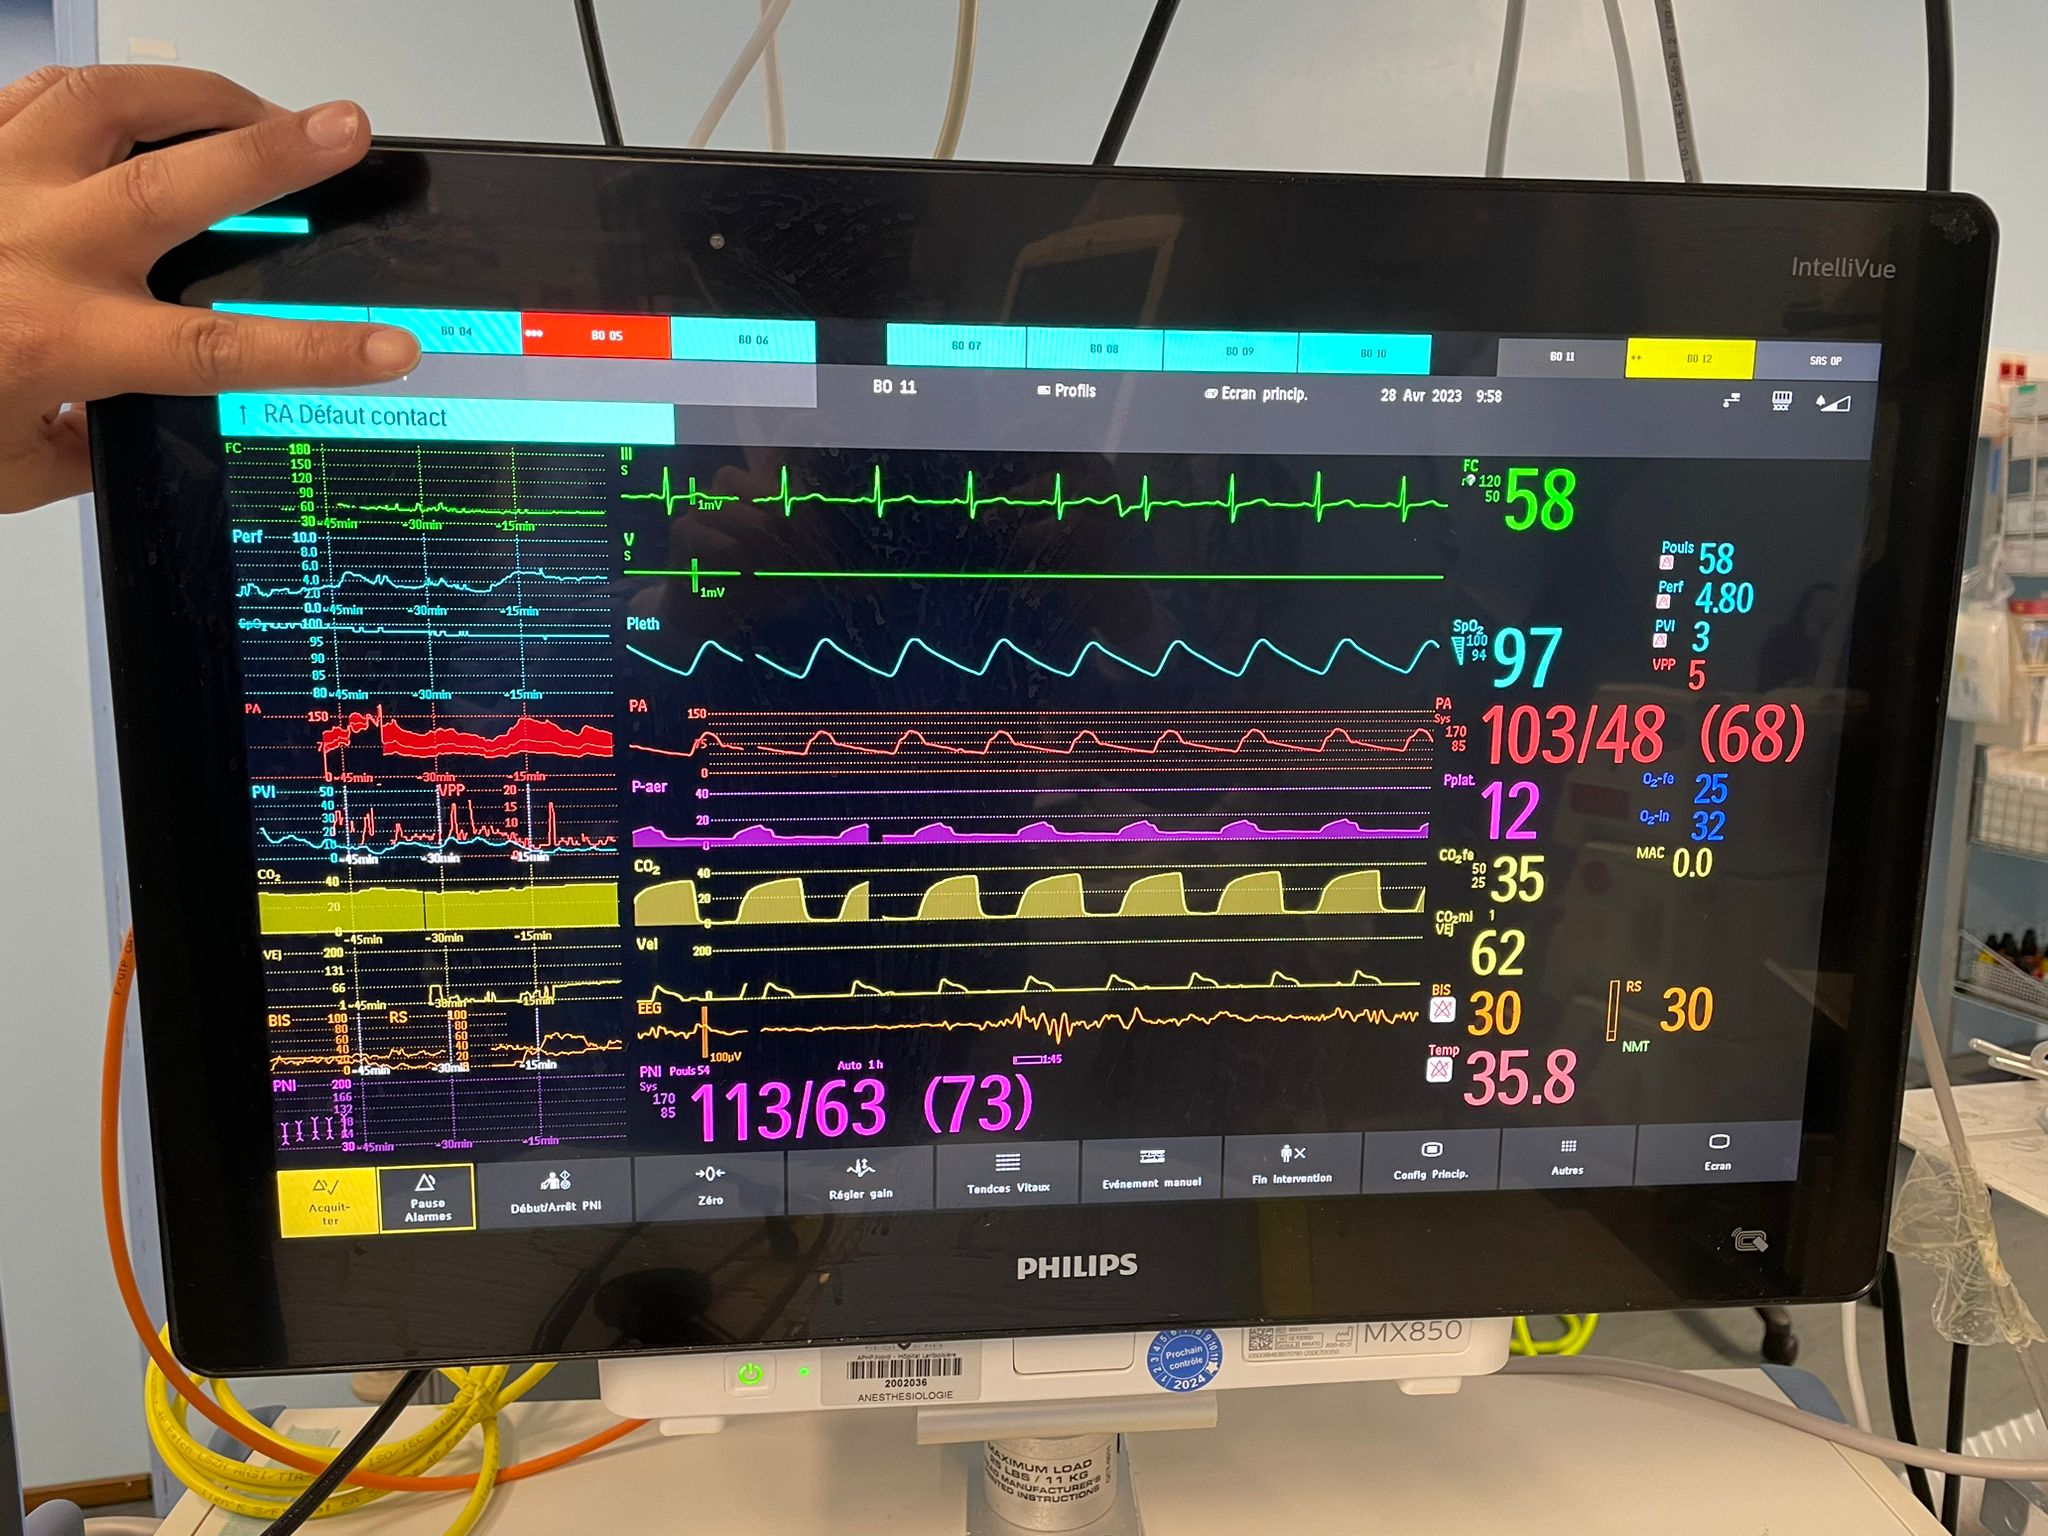
\includegraphics[
            width=1.16\paperwidth
        ]{GA_monitor_1}
    \end{picture}
}
\frame{
    \frametitle{General Anesthesia Monitoring}


    \begin{tikzpicture}[overlay, remember picture]
            \node[anchor=center, white, xshift=-32ex, yshift=-6em] at (current page.north) (ECG) {\highlight[shadow=false]{\Large \bf ECG}};
            \node[anchor=center, white, xshift=-13ex, yshift=-7.5em] at (current page.north) (ECG_head) {};
            \draw[->, very thick, white] (ECG.east) -- (ECG_head);

            \node[anchor=center, white, xshift=-32ex, yshift=-9.5em] at (current page.north) (Pleth) {\highlight[shadow=false]{\Large \bf Pleth.}};
            \node[anchor=center, white, xshift=-11ex, yshift=-10.5em] at (current page.north) (Pleth_head) {};
            \draw[->, very thick, white] (Pleth.east) -- (Pleth_head);

            \node[anchor=center, white, xshift=-32ex, yshift=-13.5em] at (current page.north) (Resp) {\highlight[shadow=false]{\Large \bf Resp.}};
            \node[anchor=center, white, xshift=-7ex, yshift=-15em] at (current page.north) (Resp_head) {};
            \draw[->, very thick, white] (Resp.east) -- (Resp_head);

            \node[anchor=center, white, xshift=-32ex, yshift=-16.5em] at (current page.north) (EEG) {\highlight[shadow=false]{\Large \bf EEG}};
            \node[anchor=center, white, xshift=-5ex, yshift=-17.5em] at (current page.north) (EEG_head) {};
            \draw[->, very thick, white] (EEG.east) -- (EEG_head);
            \node[anchor=north west, xshift=18ex, yshift=-6em] at (current page.north) {
                \highlight[shadow=false]{Indicators}
            };

    \end{tikzpicture}

    \visible<2>{
    \centering
    \highlight{\parbox{.45\textwidth}{
        \centering
        Find predictive representations of multivariate signals\\using AI.
    }}\\
    }
}

}

%------------------------------------------------------------------------------
\frame[t]{
    \frametitle[t]{Recent breakthrough in AI: Foundation Models}

    \begin{columns}[T]
        \column{.2\textwidth}\centering
        
\includegraphics[height=4em]{logo_chatGPT}\\
        \textbf{ChatGPT}
        % \column{.2\textwidth}\centering
        % 
\includegraphics[height=4em]{logo_copilot}\\
        % \textbf{Copilot}
        \column{.2\textwidth}\centering
        
\includegraphics[height=4em]{logo_midjourney}\\
        \textbf{Midjourney}
    \end{columns}
    \vskip1em
    {\centering \large What do they have in common?\\}

    \pause

    \vskip1em
    \begin{columns}[T]
        \techterm{Tokens}
        \techterm{Self-supervised pretraining}
    \end{columns}
    \vskip1em
    {\centering Capture the input distribution $\mathbb P(X)$ with interaction between tokens.\\}

    \only<3>{
        \vskip1em
        {\bf Challenges for signals:}\\[1em]

        \begin{itemize}\itemsep.5em
            % \item Which pretext task to use to capture the signals' distribution?
            \item What are the tokens of the signals?
            \item How to derive more interpretable models?
        %     \item Smaller Databases compared to Text and Images\\
        %     \item Interpretability \hskip8ex \myitem What are the tokens ?
        \end{itemize}
    }


}



%------------------------------------------------------------------------------
{
\usebackgroundtemplate{
    \begin{picture}(400, 300)(45, 0)
        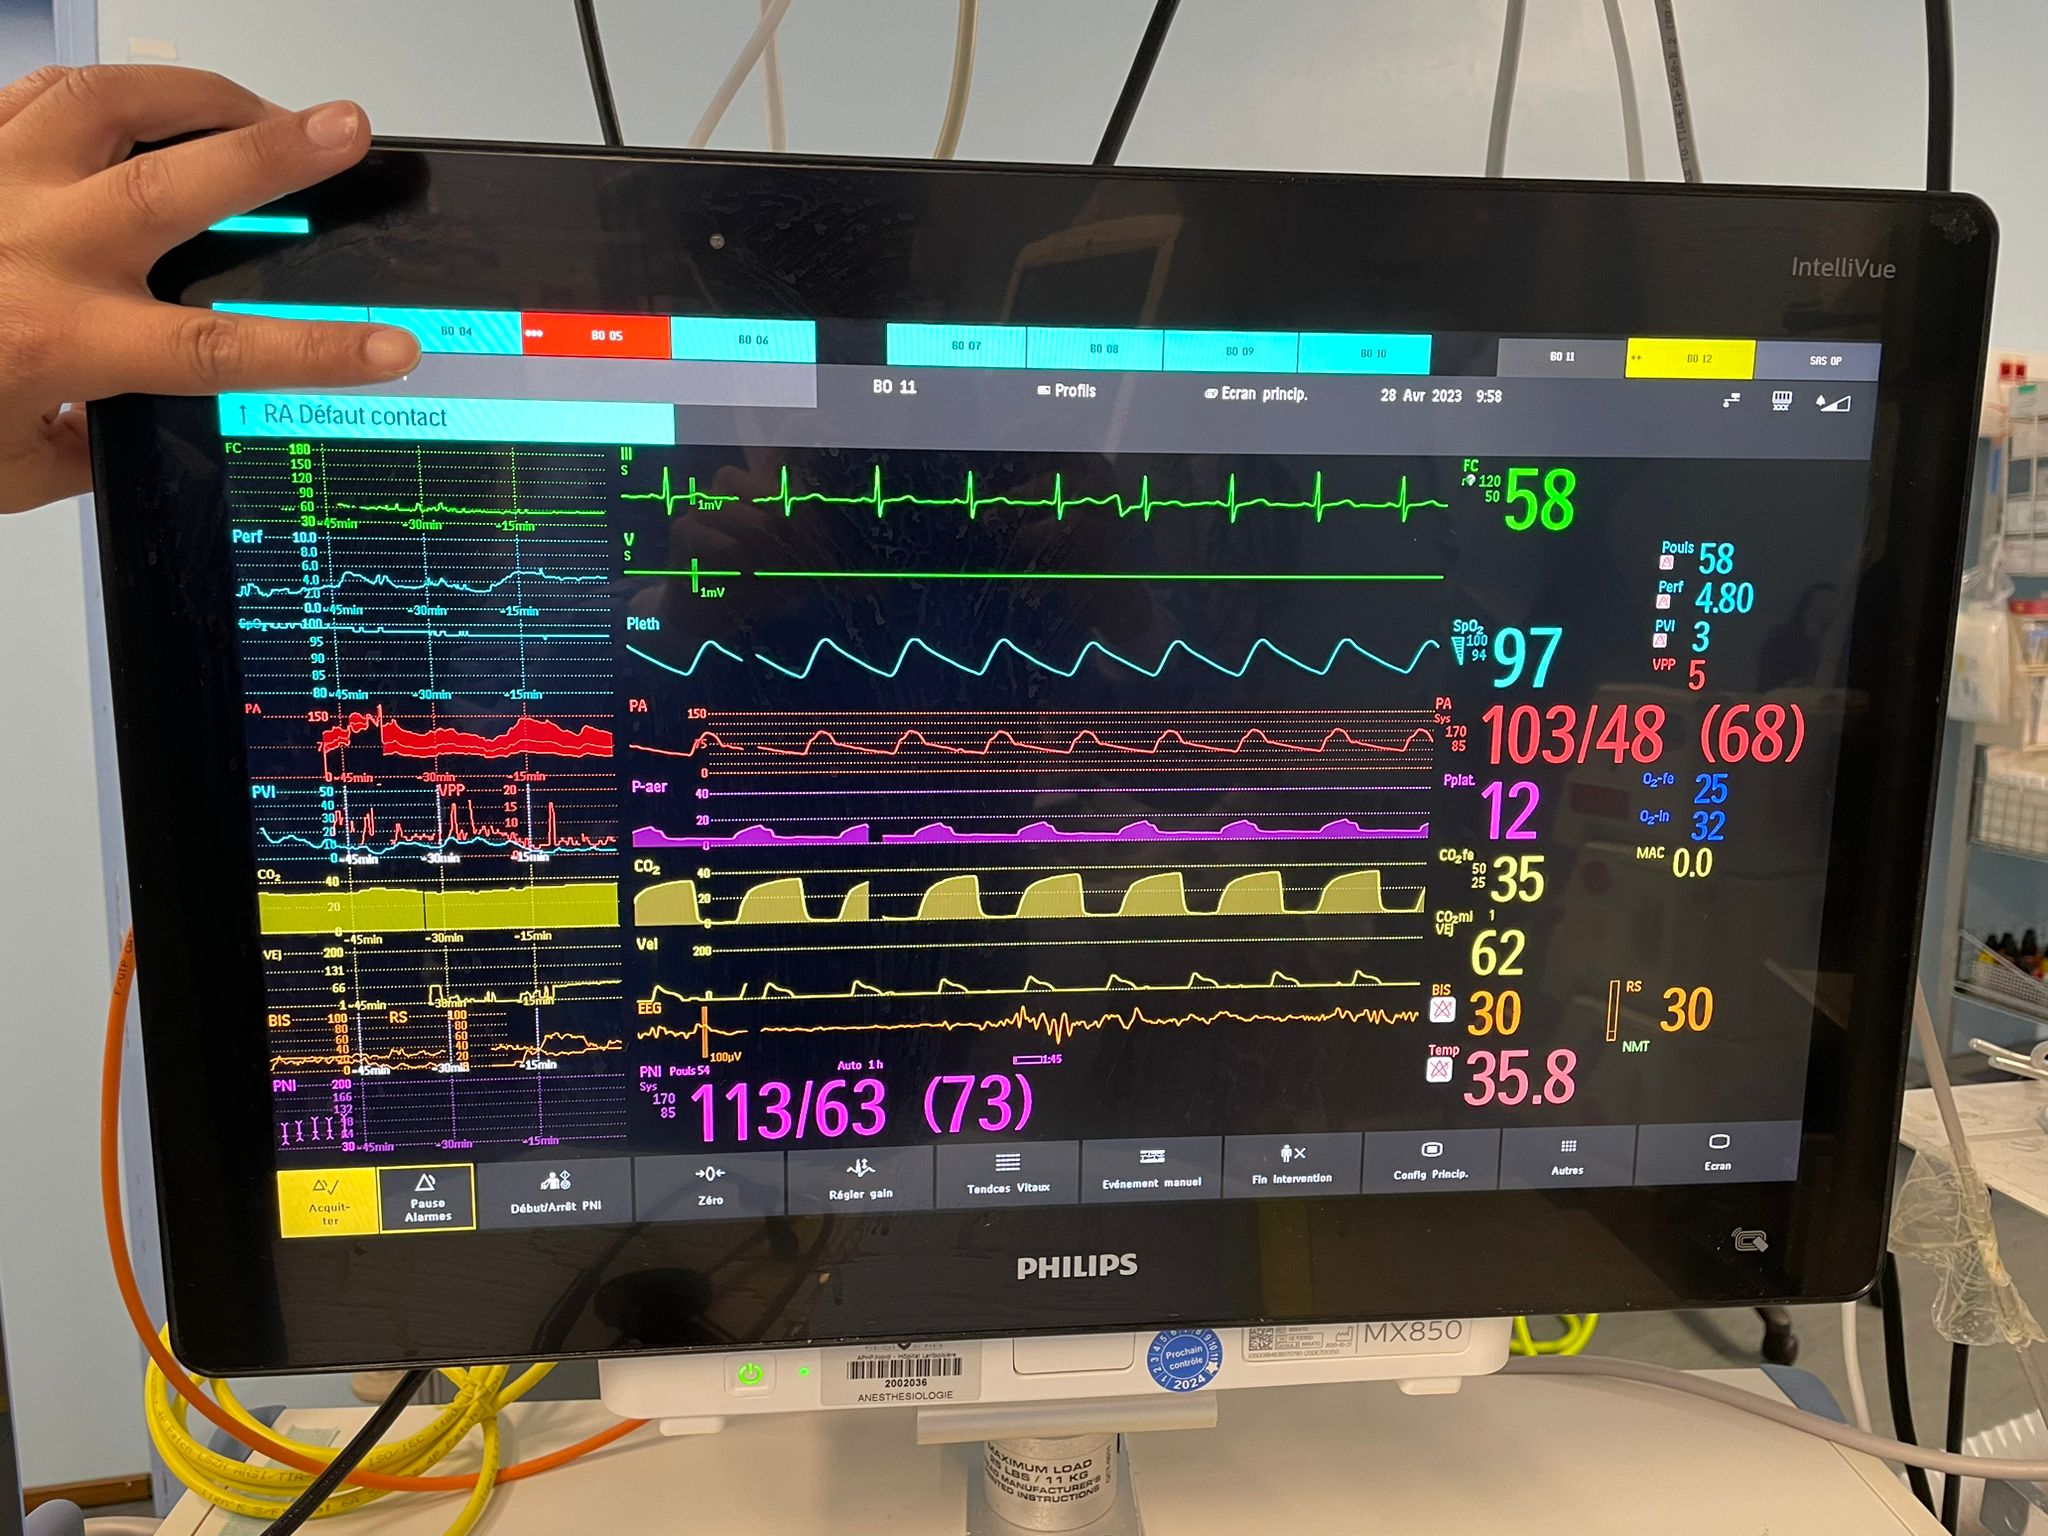
\includegraphics[
            width=1.16\paperwidth
        ]{GA_monitor_1}
    \end{picture}
}
\frame{
    \frametitle{Signals' Tokens: Events}


    \setbeamercolor{events}{bg=darkred!50}
    \begin{tikzpicture}[overlay, remember picture]

        \visible<2->{
        \node[anchor=east, yshift=7em, xshift=-3em] at (current page.east)
            (patterns) {\highlight[shadow=false]{
                % Signal's patterns
                % Underlying events
                Latent events
            }};

        \node[anchor=east, yshift=-2.5em] at (patterns.east) (ECG) {\highlight[shadow=false]{\color{black}\normalfont Heartbeat}};

        \node[rectangle, lightblue!70, draw=lightblue!70, very thick,
            minimum width=5ex,
            minimum height=2em, xshift=5.5ex, yshift=-7.8em]
                at (current page.north) (box_ecg) {};
        \draw[->, ultra thick, lightblue!70] ($(ECG.west)+(3ex, 0)$) -- (box_ecg.east);
        \node[anchor=south, xshift=.2ex, yshift=1em] at (box_ecg.west) (ecg_tip) {};
        \node[anchor=south, xshift=.2ex, yshift=-.8em] at (box_ecg.west) (ecg_base) {};
        \draw[-{Square[]}, ultra thick, green] (ecg_base) -- (ecg_tip) ;



        \node[anchor=east, yshift=-5em] at (patterns.east) (Pleth) {\highlight[shadow=false]{\color{black}\normalfont  Dichrote wave}};

        \node[rectangle, lightblue!70, draw=lightblue!70, very thick,
            minimum width=4ex,
            minimum height=2em, xshift=.2ex, yshift=-10.8em]
                at (current page.north) (box_pleth) {};
        \draw[->, ultra thick, lightblue!70] ($(Pleth.west)+(3ex, 0)$) -- (box_pleth.east);
        \node[anchor=south, xshift=.1ex, yshift=1.5em] at (box_pleth.west) (pleth_tip) {};
        \node[anchor=south, xshift=.1ex, yshift=-1em] at (box_pleth.west) (pleth_base) {};
        \draw[-{Circle[]}, ultra thick, blue] (pleth_base) -- (pleth_tip) ;

        \node[anchor=east, yshift=-7.5em] at (patterns.east) (Resp) {\highlight[shadow=false]{\color{black}\normalfont  Breath Cycle}};

        \node[rectangle, lightblue!70, draw=lightblue!70, very thick,
        minimum width=4ex,
        minimum height=2em, xshift=-2ex, yshift=-15.5em]
        at (current page.north) (resp_box) {};
        \draw[->, ultra thick, lightblue!70] ($(Resp.west)+(3ex, 0)$) -- (resp_box.east);
        \node[anchor=south, xshift=.2ex, yshift=1.5em] at (resp_box.west) (resp_tip) {};
        \node[anchor=south, xshift=.2ex, yshift=-1em] at (resp_box.west) (resp_base) {};
        \draw[-{Triangle[]}, ultra thick, yellow] (resp_base) -- (resp_tip) ;

        \node[anchor=east, yshift=-10em] at (patterns.east) (EEG) {\highlight[shadow=false]{\color{black}\normalfont  Brain waves}};

        \node[rectangle, lightblue!70, draw=lightblue!70, very thick,
        minimum width=6ex,
        minimum height=1.3em, xshift=-2ex, yshift=-17.8em]
        at (current page.north) (eeg_box) {};
        \draw[->, ultra thick, lightblue!70] ($(EEG.west)+(3ex, 0)$) -- (eeg_box.east);
        \node[anchor=south, xshift=.2ex, yshift=1.5em] at (eeg_box.west) (eeg_tip) {};
        \node[anchor=south, xshift=.2ex, yshift=-.6em] at (eeg_box.west) (eeg_box) {};
        \draw[-{Turned Square[]}, ultra thick, orange] (eeg_box) -- (eeg_tip) ;
        }



        \node[anchor=west, xshift=0em, yshift=7em] at (current page.west)
            (events) {\highlight[shadow=false, col=events,c=white]{
                Observed events
            }};
        \node[anchor=west, yshift=-3.5em] at (events.west)
            {\highlight[shadow=false,col=events,c=black]{
                \normalfont Drug injection
            }};
        \node[anchor=west, yshift=-7em] at (events.west)
            {\highlight[shadow=false,col=events,c=black]{
                \normalfont Surgery acts
            }};
        \node[anchor=west, yshift=-10.5em] at (events.west)
            {\highlight[shadow=false,col=events,c=black]{
                \normalfont Adverse outcomes
            }};
        \node[anchor=west, yshift=-14em] at (events.west)
            {\highlight[shadow=false,col=events,c=black]{
                \normalfont Stimulus
            }};

    \end{tikzpicture}
}
}


%------------------------------------------------------------------------------

\begin{frame}[t]{Signals' Tokens: Events}

    \vskip-1em
    \begin{columns}[T]
        \column{.5\textwidth}
        \centering
        \begin{tikzpicture}
                \node[inner sep=0em, outer sep=0em] (img) {\includegraphics[width=.9\linewidth]{meg_signal}};
                \path let
                  \p1=($(img.north) - (0, 1em)$), \p2=(img.south)
                  in
                  node {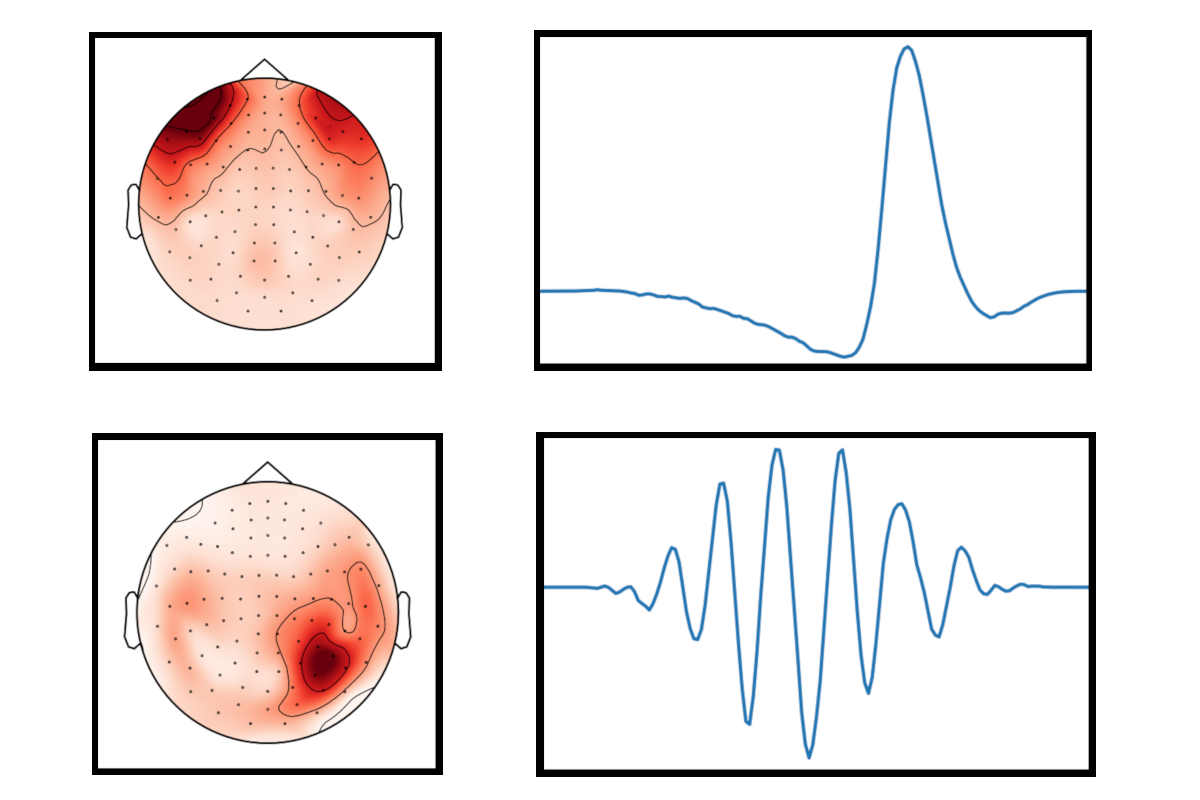
\includegraphics[height=\y1-\y2]{meg_dict}};
            \end{tikzpicture}\\
        {\large Neuroscience (MEG)}\\[1em]
        \begin{tikzpicture}
            \node[inner sep=0em, outer sep=0em] (img) {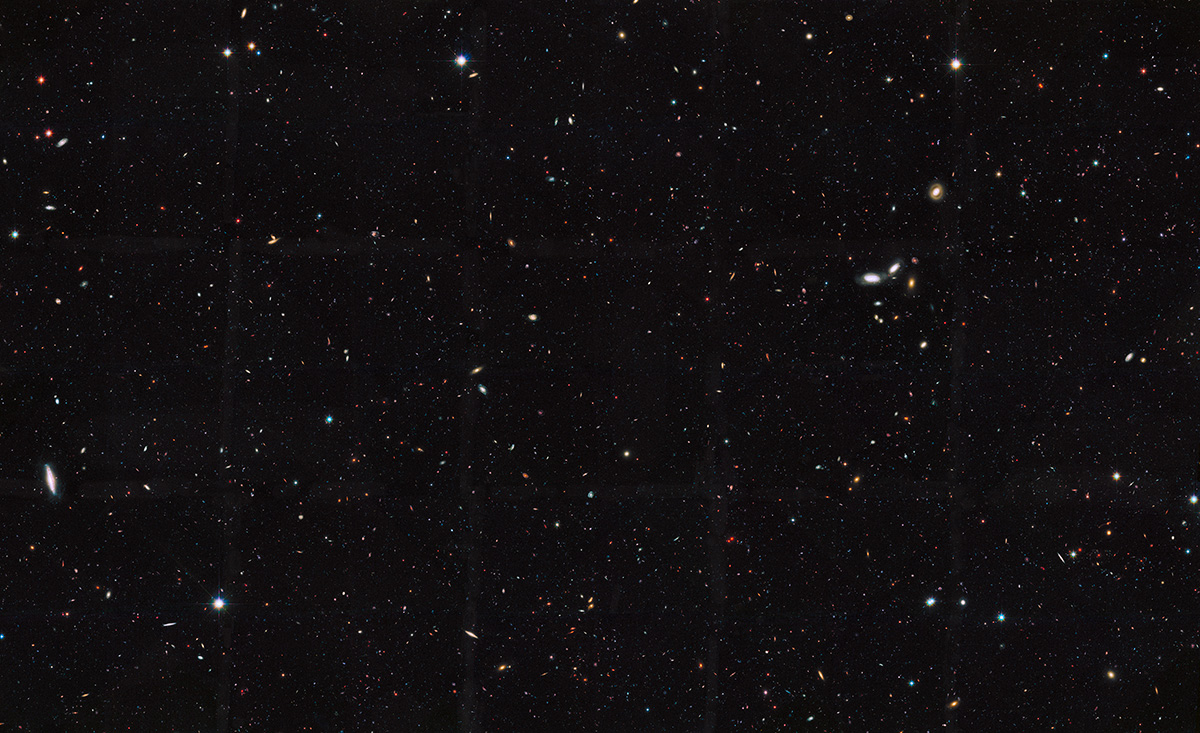
\includegraphics[width=.9\linewidth]{Hubble}};
            \path let
                \p1=($(img.north) - (0, 1em)$), \p2=(img.south)
                in
                node {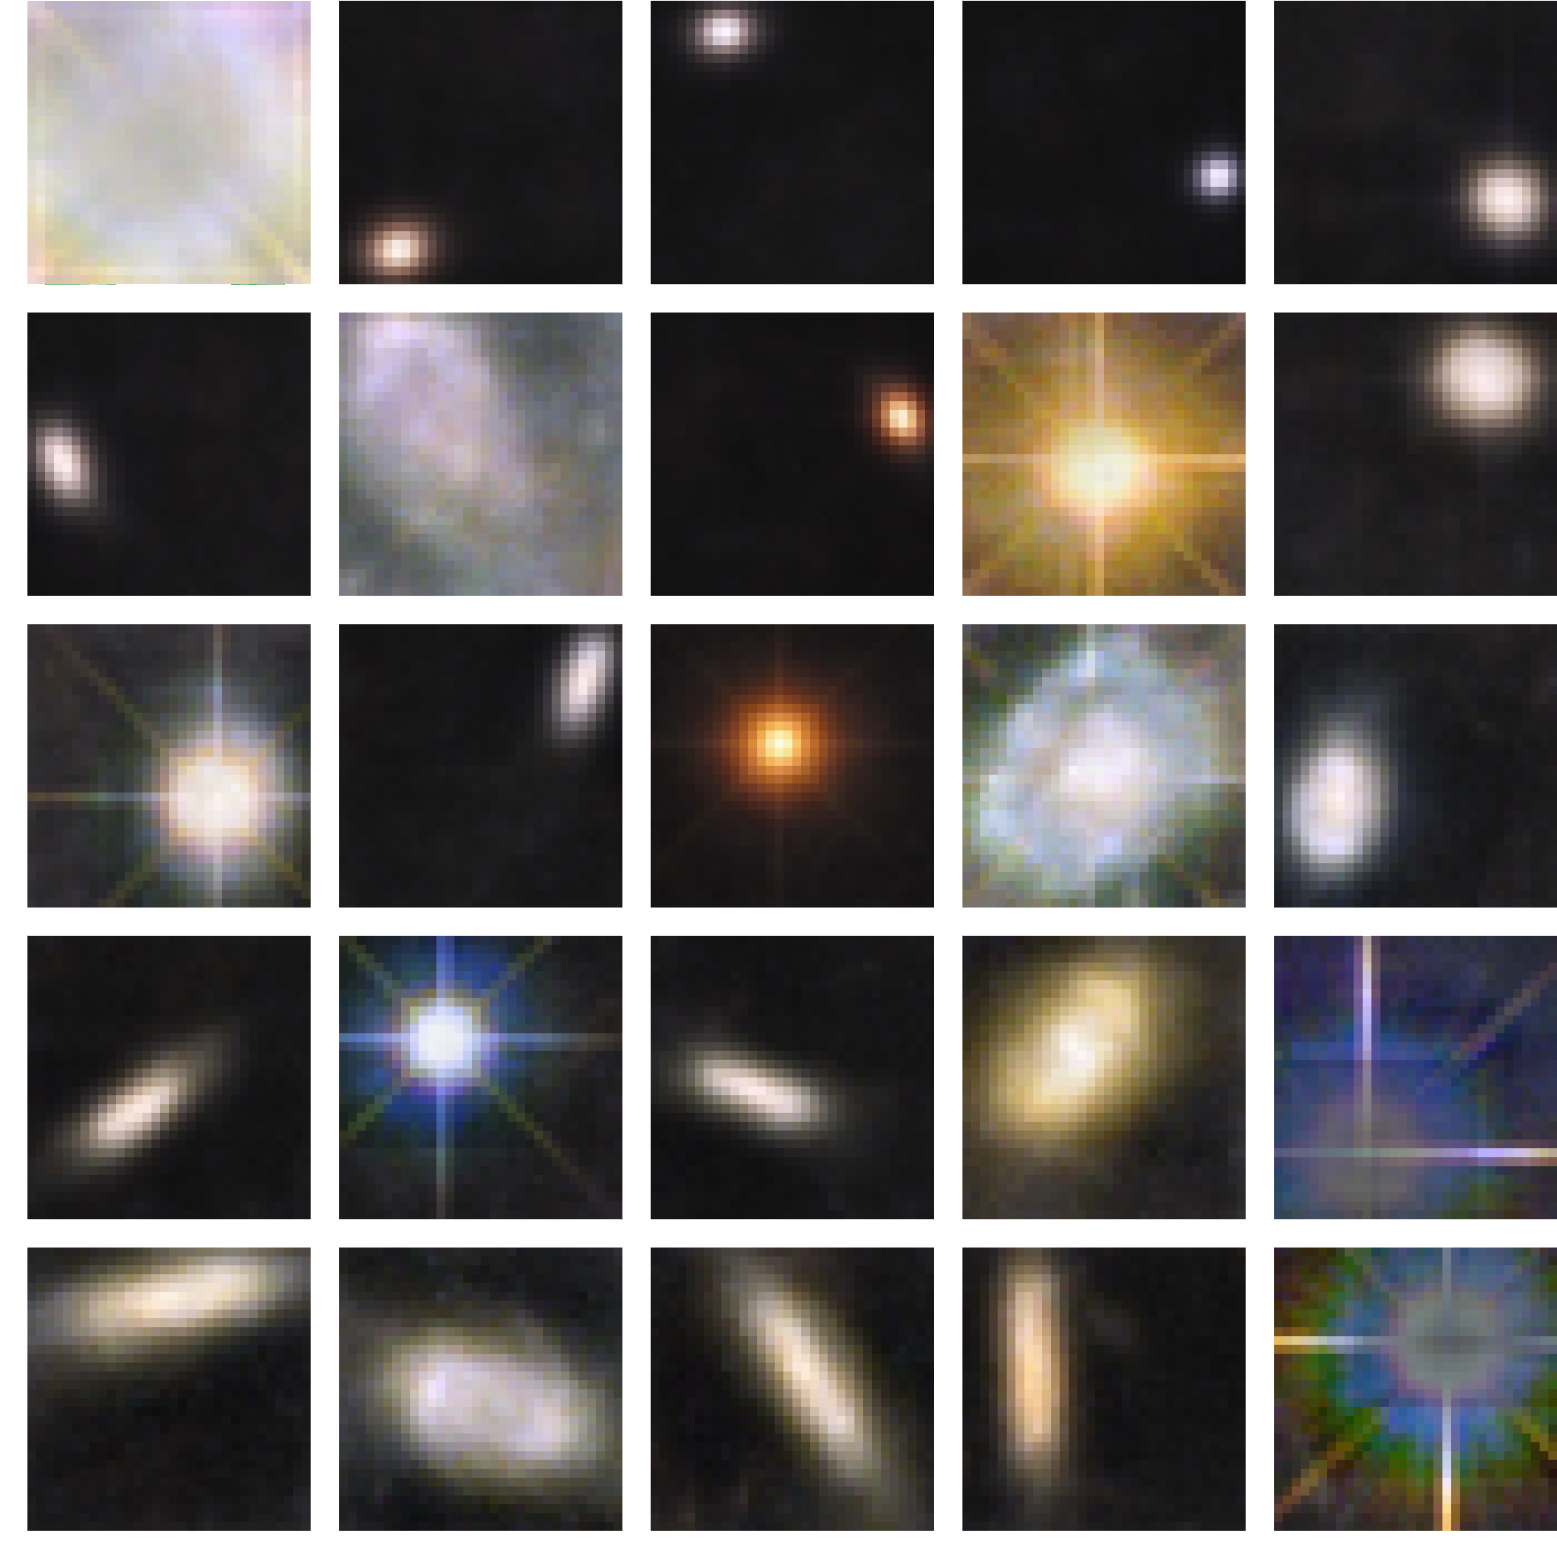
\includegraphics[height=\y1-\y2]{Hubble_dict}};
        \end{tikzpicture}\\
        {\large Astronomy}\\
    \column{.5\textwidth}
        \centering
        \begin{tikzpicture}
            \node[inner sep=0em, outer sep=0em] (img) {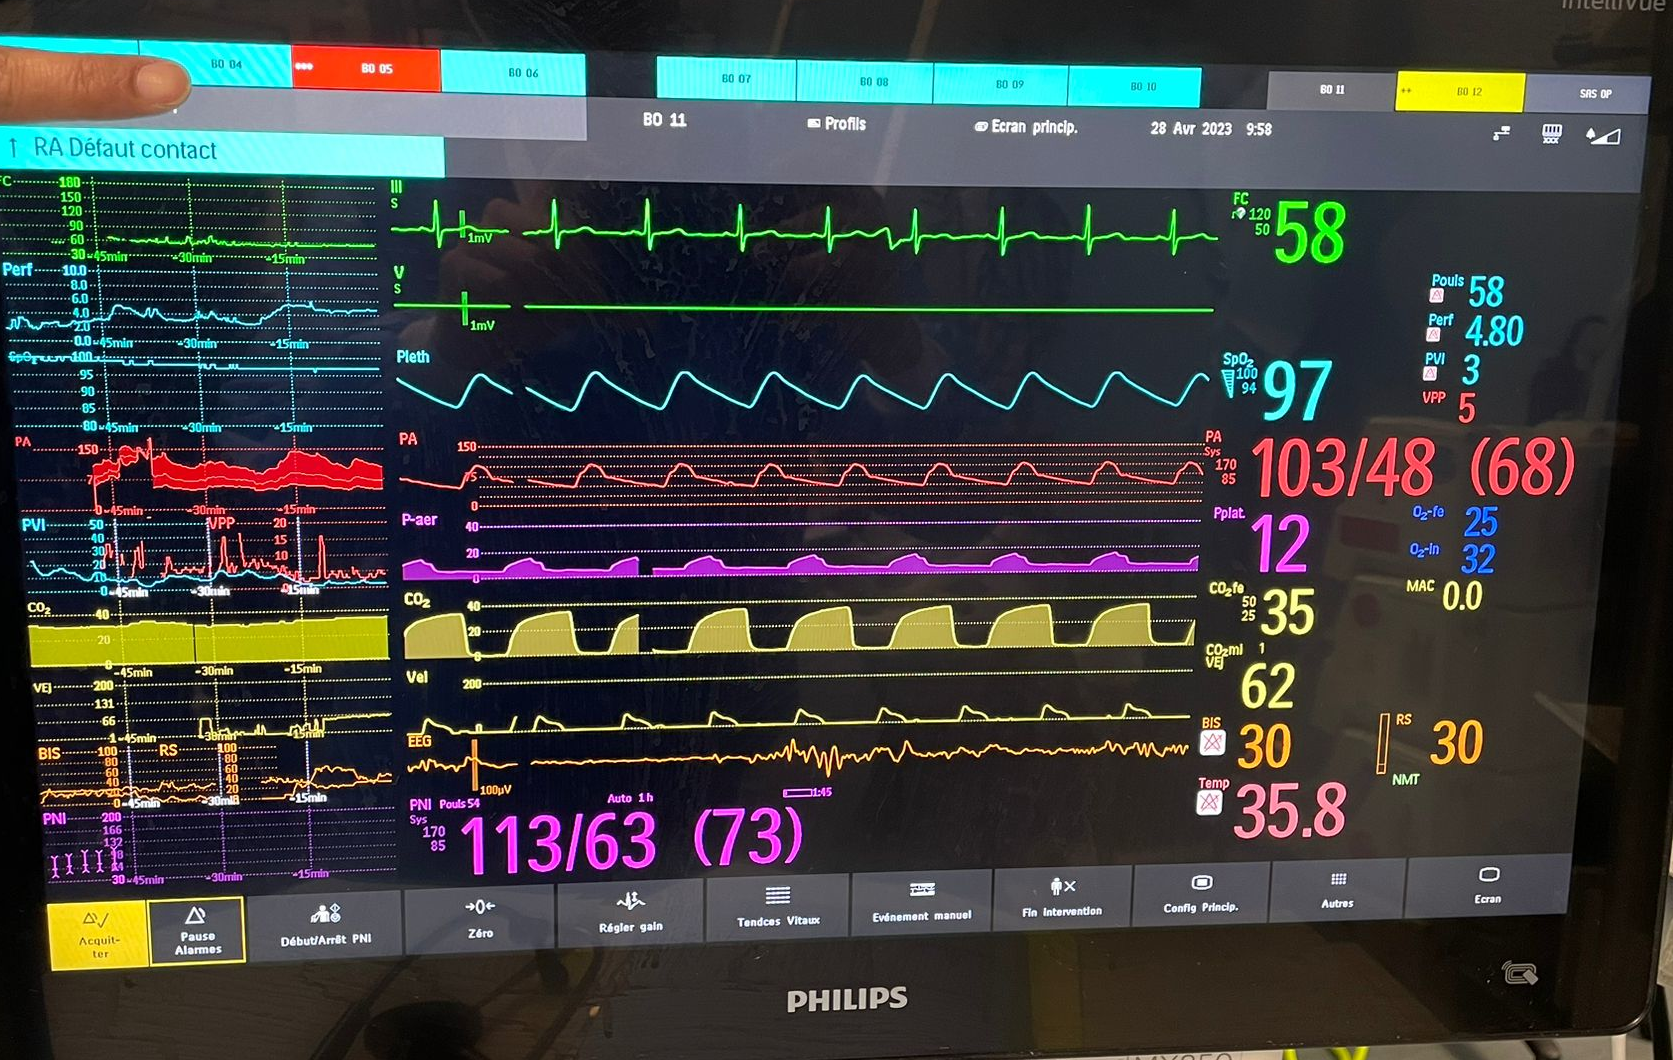
\includegraphics[width=.8\linewidth]{ga_signal}};
            \path let
                \p1=($(img.north) - (0, 1em)$), \p2=(img.south)
                in
                node {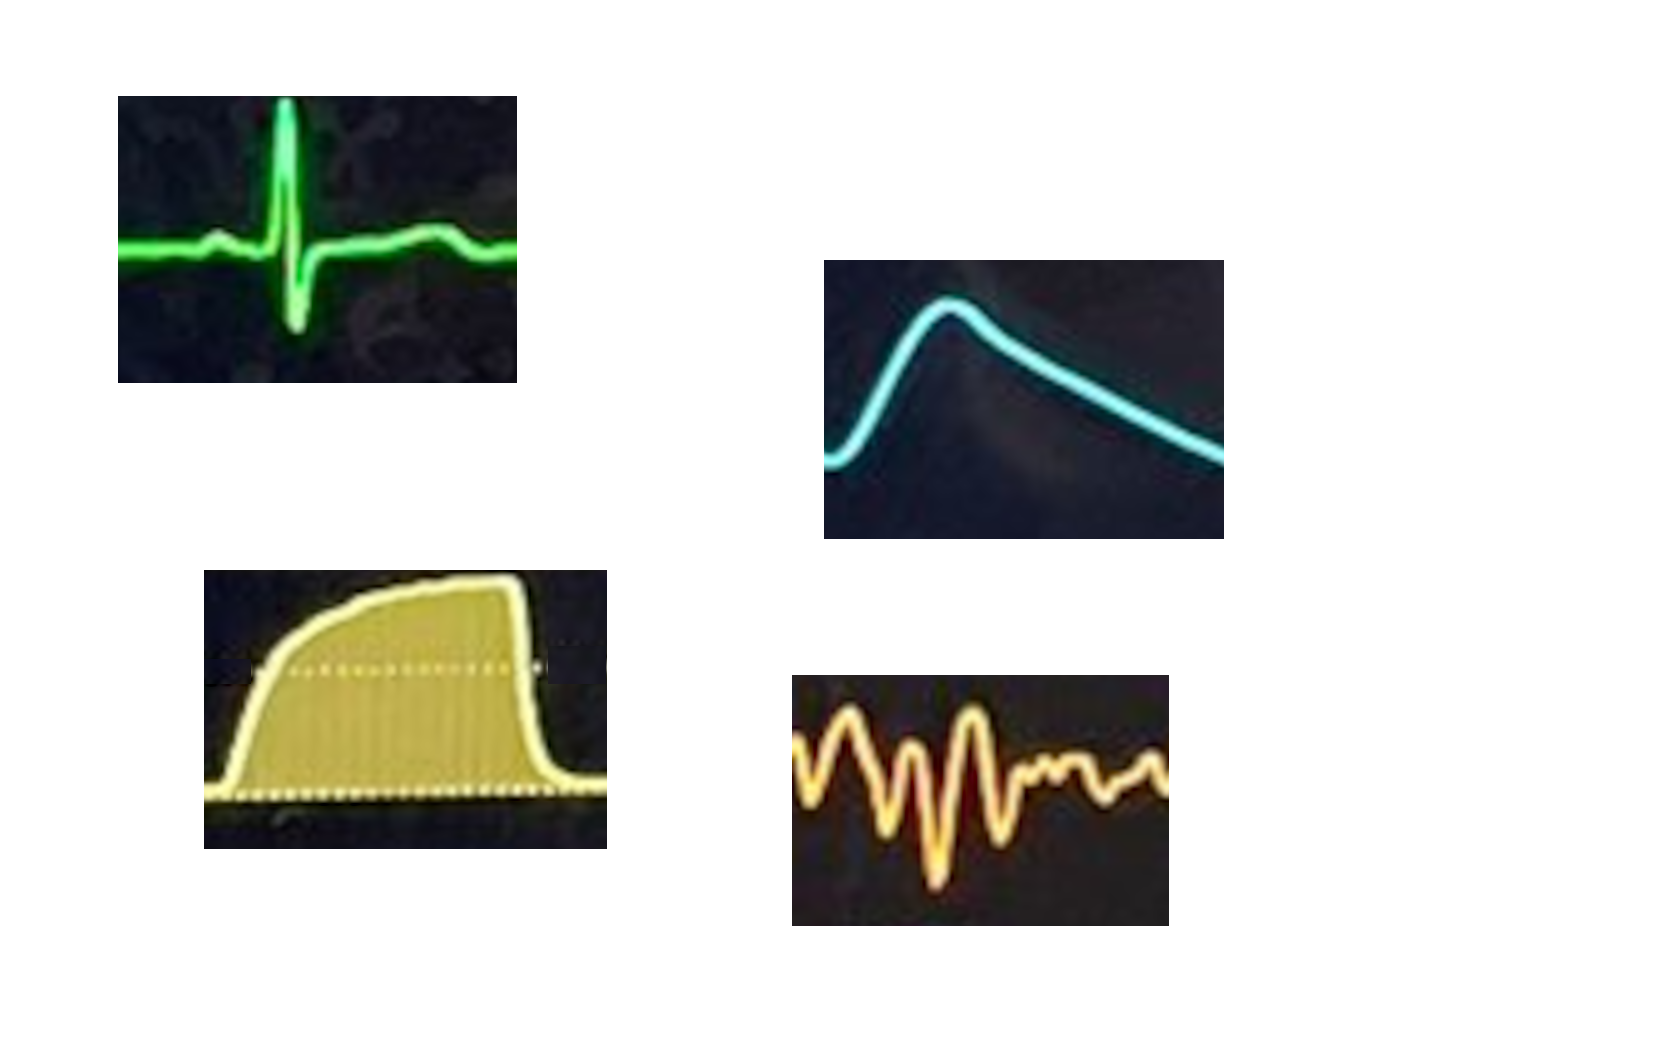
\includegraphics[height=\y1-\y2]{ga_dict}};
        \end{tikzpicture}\\
        {\large General Anesthesia}\\[1em]
        \begin{tikzpicture}
            \node[inner sep=0em, outer sep=0em] (img) {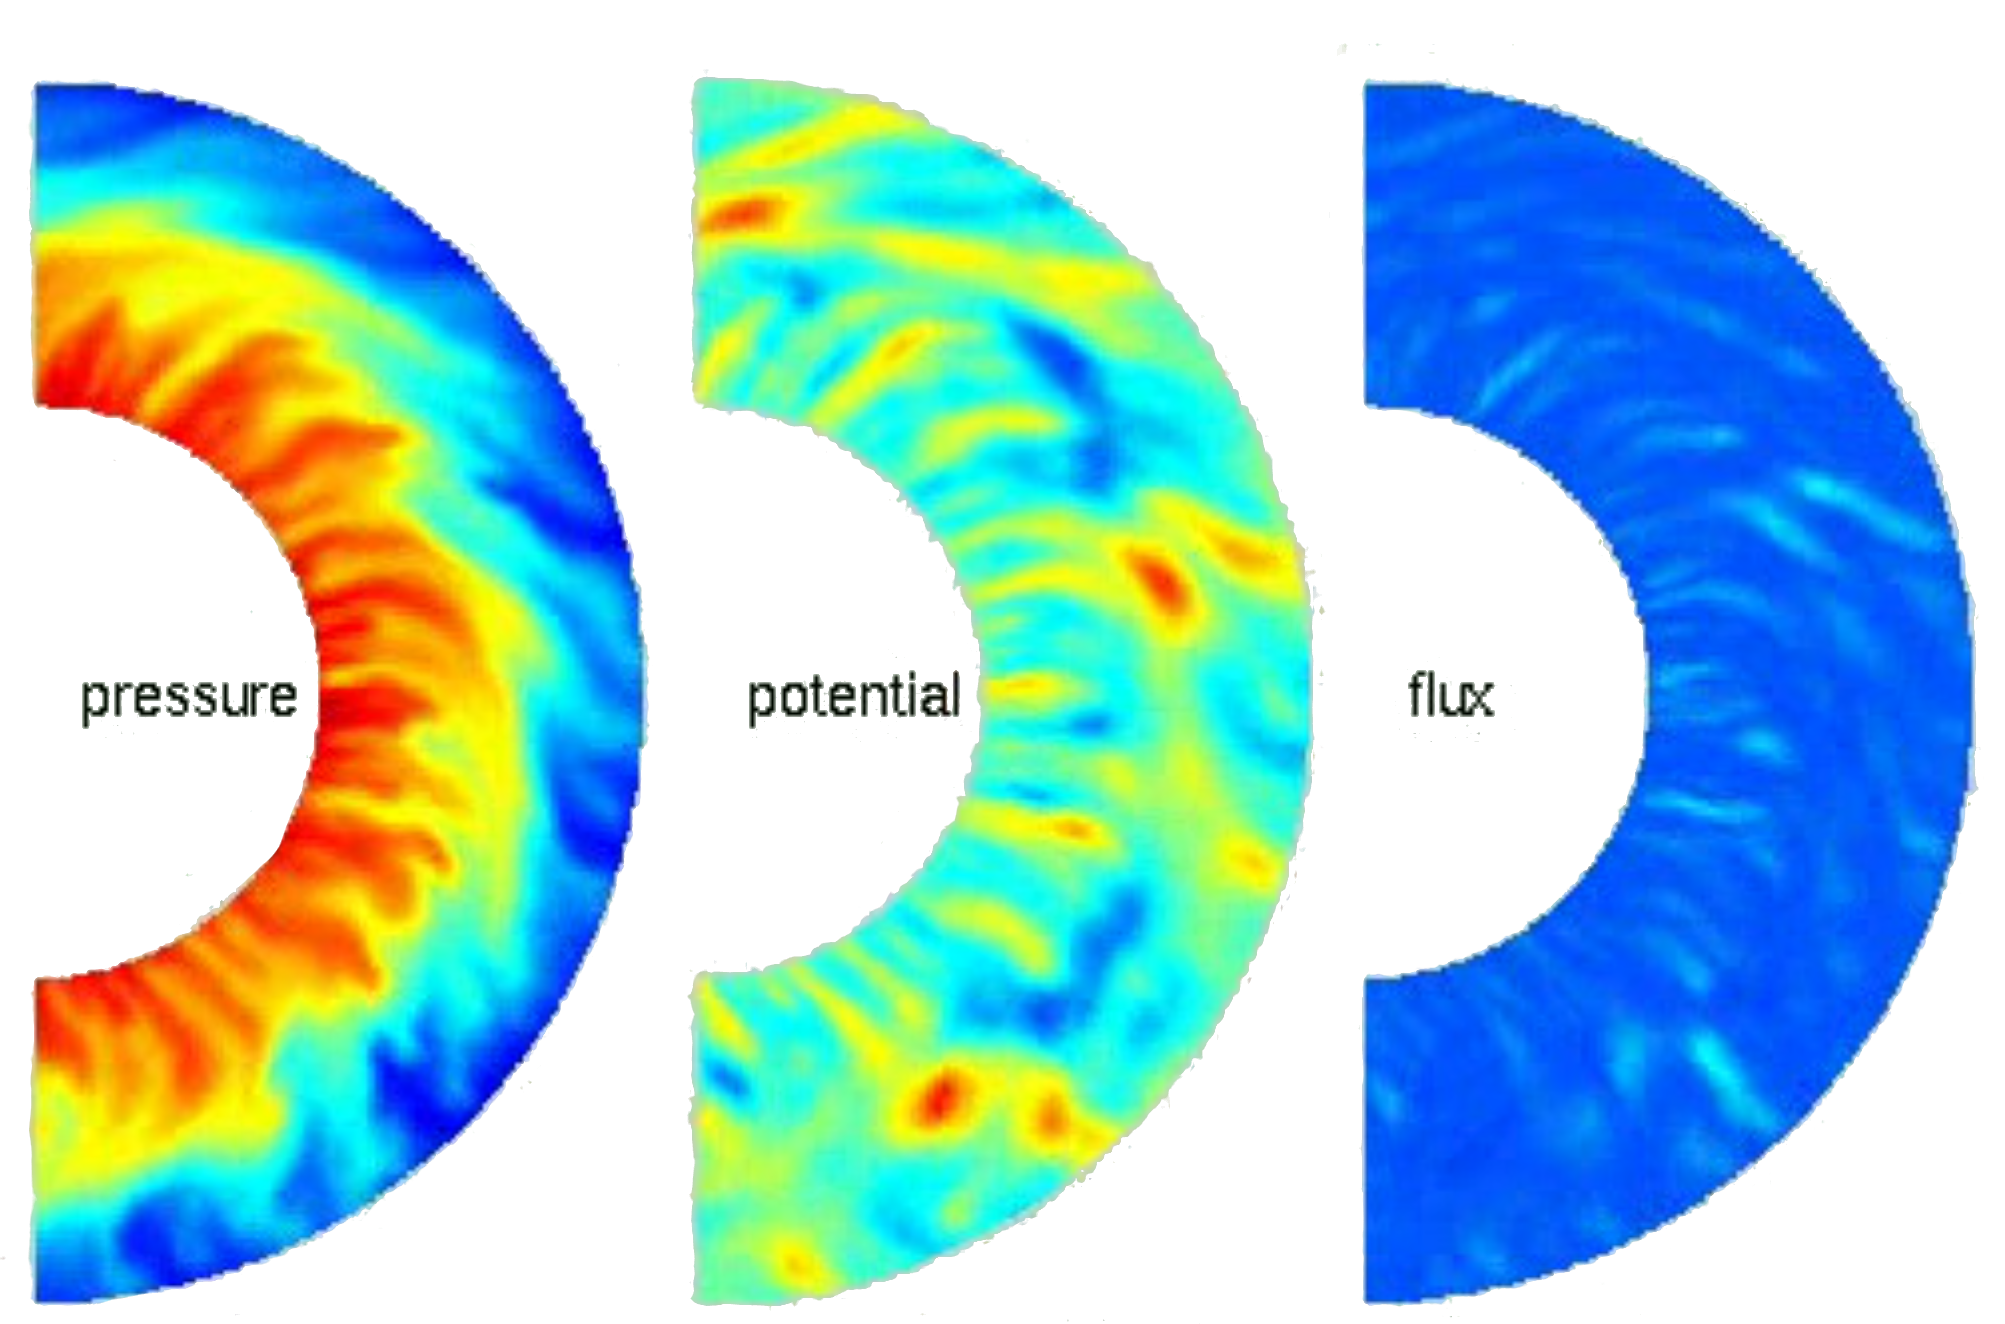
\includegraphics[width=.9\linewidth]{tokamak}};
            \path let
                \p1=($(img.north) - (0, 1em)$), \p2=(img.south)
                in
                node {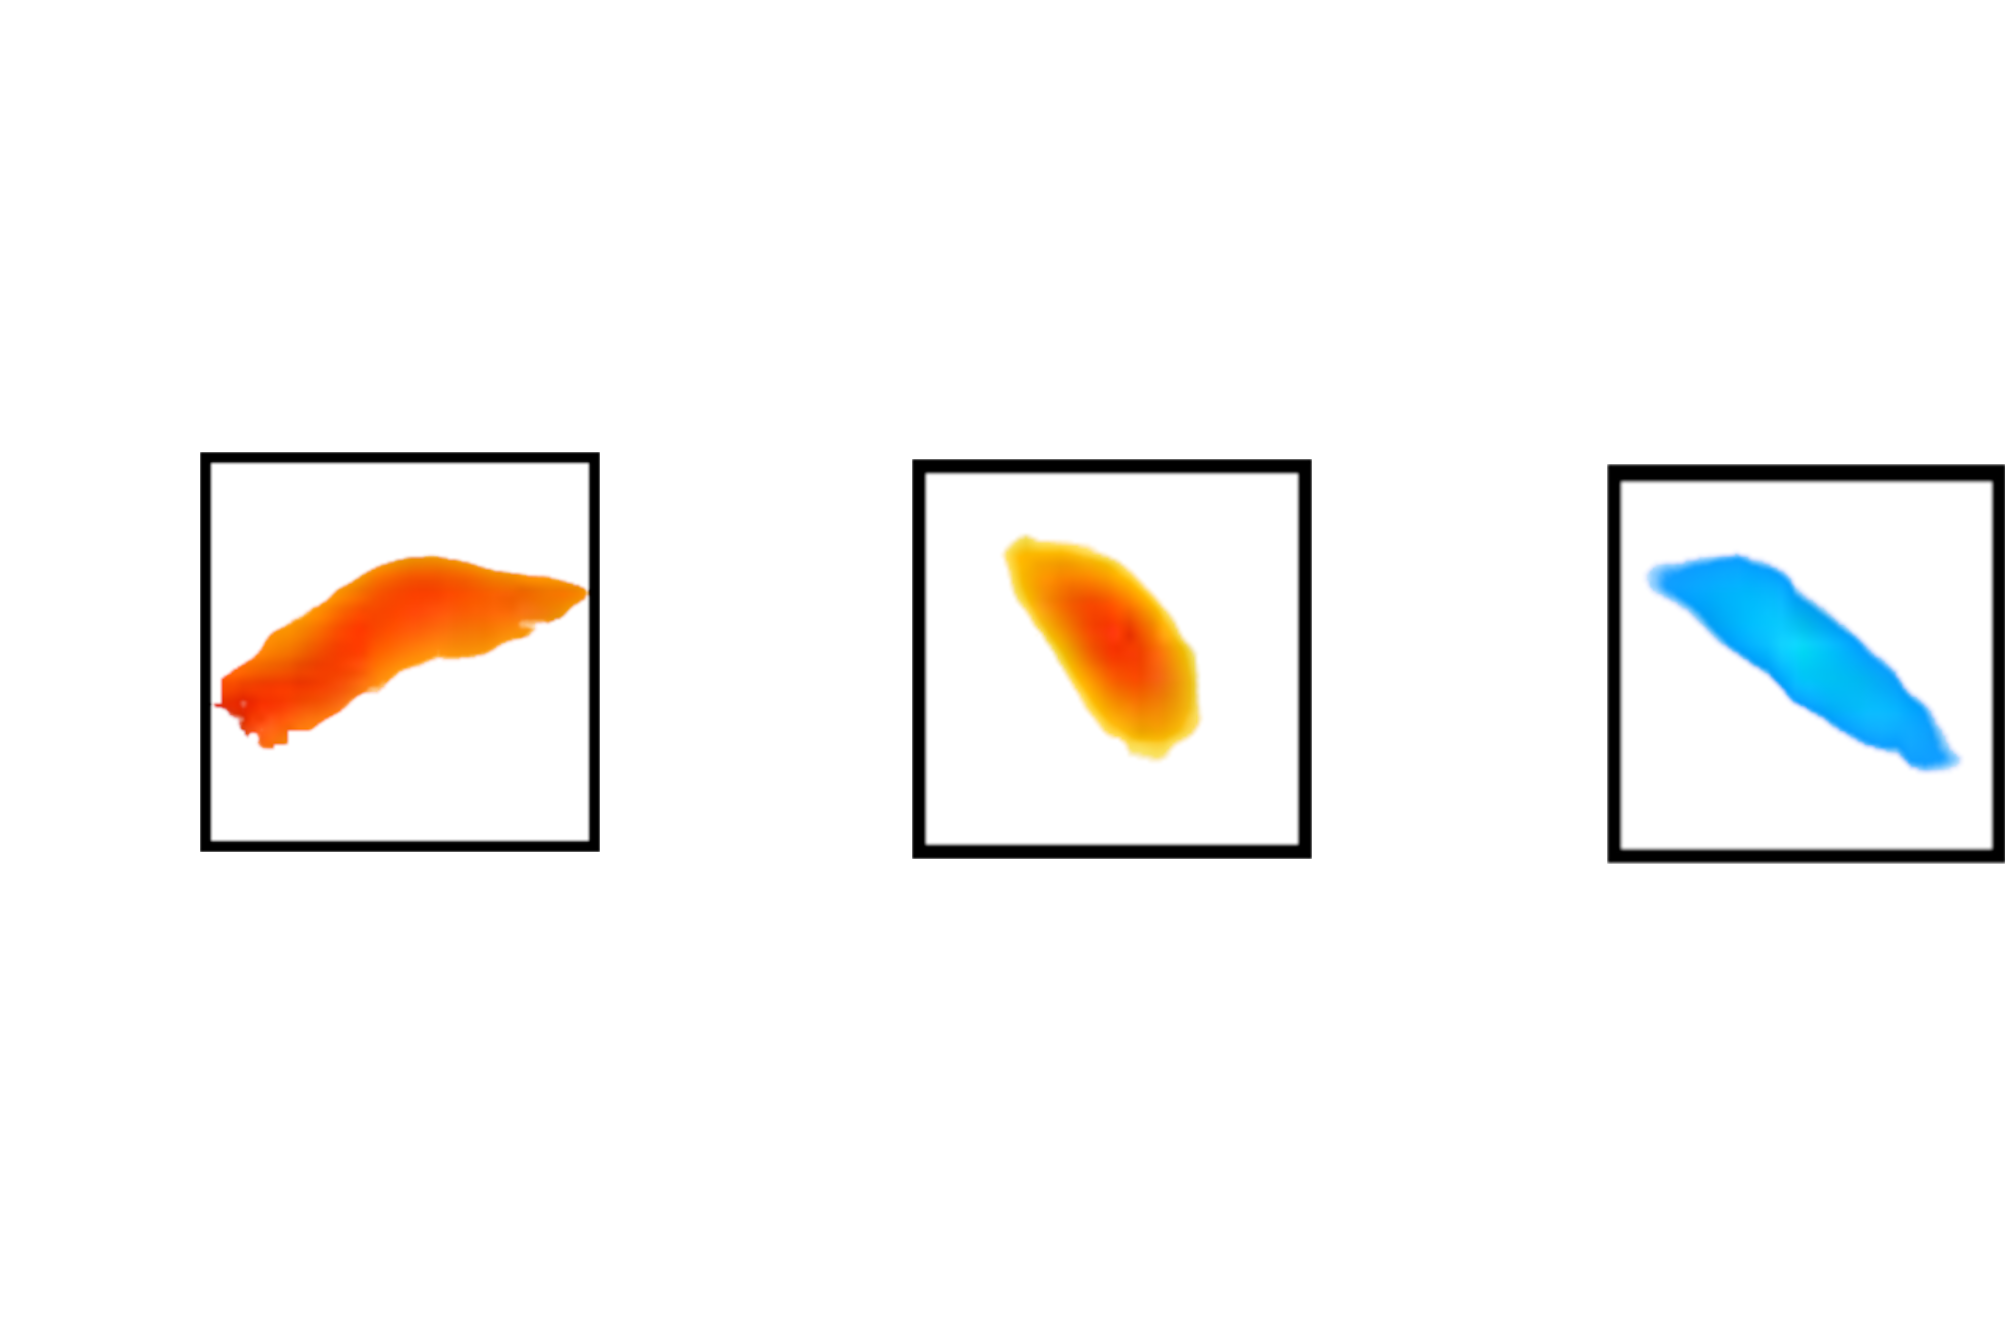
\includegraphics[height=\y1-\y2]{tokamak_dict}};
        \end{tikzpicture}\\
        {\large Physics Simulation}\\

    \end{columns}

    % \visible<2>
    {\vskip-14em
    \centering
    \highlight{\parbox{.35\textwidth}{
        \centering
        Latent Events\\
        are characterized by
        Recurring Patterns
    }}\\
    }
\end{frame}


%------------------------------------------------------------------------------

\frame{
    \frametitle{EULPS: Event-based Unsupervised Learning for Physiological Signals}


    \begin{block}{\bf EULPS Goal}
        Model Physiological Signals as a Distribution of Events.
    \end{block}

    \vskip1em

    % {\bf Hyp.:} Events' time distribution $\mathbb P(\{t_k\}_k)$ is much simpler than $\mathbb P(X)$.\\[1em]

    {\bf Challenge:} Need to infer what are the events and model their distribution jointly.\\[1em]

    {\centering
\includegraphics[width=.8\textwidth]{finding_events}\\[1em]}

    % {\bf Approach:} from interpretable models to deep learning.
    \pause
    \begin{columns}
        \hskip-1ex
        \column{.3\textwidth}
        \highlight{\parbox{\textwidth}{%
            \centering Events' distribution models\phantom{g}
        }}%
        \column{.3\textwidth}
        \highlight{\parbox{\textwidth}{%
            \centering Joint Modeling of Signals and Events
        }}%
        \column{.3\textwidth}
        \highlight{\parbox{\textwidth}{%
            \centering Task-specific Fine-tuning Algo.
        }}%
    \end{columns}
}

% \frame[t]{
%     \frametitle{EULPS: Event-based Unsupervised Learning for Physiological Signals}

%     \vskip-.5em
%     \highlight{
%         \centering Goal: \normalfont\normalcolor
%          Propose a new Signal Processing methodology based on Events.
%     }

%     % tikz figure with 3 circles linked with arrows going forward and backward and the the following text in each circle:
%     % - Core ML
%     %- Applications
%     % - Software
%     \setbeamercolor{dl}{fg=white,bg=darkred!50}
%     \begin{tikzpicture}[overlay, remember picture]

%         \node[anchor=south, yshift=3em, xshift=-3ex] at (current page.south) (cloud_soft) {
\includegraphics[width=15ex]{cloud}};
%         \node[anchor=north, yshift=1.2em] at (cloud_soft) (Soft) {\parbox{.16\textwidth}{\centering Open\\ Source}};
%         \node[anchor=south, yshift=2em] at (Soft.north) {\parbox{.15\textwidth}{\centering \bf \color{darkred} Thomas Moreau}};
%         \node[anchor=south, xshift=-12ex, yshift=4em] at (Soft.north) (cloud_ML) {
\includegraphics[width=15ex]{cloud}};
%         \node[anchor=north, yshift=.7em] at (cloud_ML) (ML) {Core ML\phantom{p}};
%         \node[anchor=south, xshift=12ex, yshift=4em] at (Soft.north) (cloud_app) {
\includegraphics[width=15ex]{cloud}};
%         \node[anchor=north, yshift=.3em] at (cloud_app) (App) {Impact};

%         \draw[-latex] (cloud_app) to[bend right=5] node[above,rotate=60] {} (cloud_ML);
%         \draw[-latex] (cloud_ML) to[bend right=5] node[above,rotate=60] {} (cloud_app);
%         \draw[-latex] (cloud_app) to[bend right=5] node[above,rotate=60] {} (cloud_soft);
%         \draw[-latex] (cloud_soft) to[bend right=5] node[above,rotate=60] {} (cloud_app);
%         \draw[-latex] (cloud_soft) to[bend right=5] node[above,rotate=60] {} (cloud_ML);
%         \draw[-latex] (cloud_ML) to[bend right=5] node[above,rotate=60] {} (cloud_soft);

%         \node[anchor=east, xshift=-18ex, yshift=-6ex] at (cloud_soft.west) {\includegraphics[height=1.5em]{logo_python}};
%         \node[anchor=east, xshift=-10ex, yshift=-6ex] at (cloud_soft.west) (sklearn){\includegraphics[height=1.5em]{logo_sklearn}};
%         \node[anchor=south, xshift=-3ex, yshift=-1ex] at (sklearn.north) (contrib) {\footnotesize Contributor};
%         \node[anchor=east, xshift=1ex, yshift=2ex] at (cloud_soft.west) {\includegraphics[height=3em]{logo_joblib}};
%         \node[anchor=east, xshift=1ex, yshift=-5ex] at (cloud_soft.west) {\includegraphics[height=3em]{logo_loky}};
%         \node[anchor=west, xshift=-1ex, yshift=3ex] at (cloud_soft.east) (benchopt) {\includegraphics[height=3em]{logo_benchopt}};
%         \node[anchor=west, xshift=0ex, yshift=-4ex] at (cloud_soft.east) (alpha) {\includegraphics[height=3em]{brain_and_signals}};
%         \node[anchor=north, yshift=1ex] at (alpha.south) {\footnotesize\texttt{{\color{orange}$\pmb\alpha$}csc}};


%         \node[anchor=east, yshift=3.5em, xshift=2ex] at (cloud_ML.west) {
%             \highlight{\parbox[c]{.18\textwidth}{
%                 2018-2023\\
%                 \normalfont\color{black} 17 papers in top ML conf.
%             }}
%         };

%         \node[anchor=south, yshift=0em, xshift=0ex] at (cloud_app.north) {
%             \highlight{\parbox[c]{.28\textwidth}{
%                 GA Database\\
%                 \normalfont\color{black}
%                 46k recordings; 25Tb
%             }}
%         };
%         \node[anchor=west, yshift=-.5em, xshift=-3ex] at (cloud_app.east) {
%             \highlight{\parbox[c]{.25\textwidth}{
%                 Several Domains\\
%                 \normalfont \color{black}
%                 Neuroscience\\
%                 Physics Simulation\\
%                 Astrophysics
%             }}
%         };


%         \node[anchor=south, yshift=.3em] at (contrib.north) {
%             \highlight[col=dl, c=white]{\parbox{.17\textwidth}{
%                 \footnotesize \normalfont
%                 \centering {\bf Downloads:}\\
%                 26M/month
%             }}
%         };
%         \node[anchor=west, xshift=-2ex, yshift=-2em] at (benchopt.east) {
%             \highlight[col=dl, c=white]{\parbox{.15\textwidth}{
%                 \footnotesize \normalfont
%                 \centering{\bf Downloads:}\\
%                 1k/month
%             }}
%         };
%         \node[anchor=north] at (cloud_soft.south) {
%             
\includegraphics[height=1em]{github}~@tommoral
%         };
%     \end{tikzpicture}
% }





\appendix

%------------------------------------------------------------------------------
\frame{
    \frametitle{References}

    \footnotesize
    \begin{itemize}\itemindent4em
        \item[\fakecite{ICLR2022}] Allain, C., Gramfort, A. \& {\bf Moreau, T.} \emph{DriPP: Driven Point Process to Model Stimuli Induced Patterns in M/EEF Signals.} in ICLR 2022.
        \item[\fakecite{ICLR2022a}] Malézieux, B., {\bf Moreau, T.} \& Kowalski, M. \emph{Understanding approximate and Unrolled Dictionary Learning for Pattern Recovery.} in ICLR 2022.
        \item[\fakecite{NeurIPS2022}] Dagréou, M., Ablin, P., Vaiter, S. \& {\bf Moreau, T.} \emph{A framework for bilevel optimization that enables stochastic and global variance reduction algorithms.} in NeurIPS 2022.
        \item[\fakecite{ICML2023}] Staerman, G., Allain, C., Gramfort, A. \& {\bf Moreau, T.} \emph{FaDIn: Fast Discretized Inference for Hawkes Processes with General Parametric Kernels.} in ICML 2023.
        \item[\fakecite{NImg 2023}] Power, L., Allain, C., {\bf Moreau, T.}, Gramfort, A. \& Bardouille, T. \emph{Using convolutional dictionary learning to detect task-related neuromagnetic transients and ageing trends in a large open-access dataset.} NeuroImage 2023.

    \end{itemize}
}

\frame{
    \frametitle{Task Table}

    \centering
    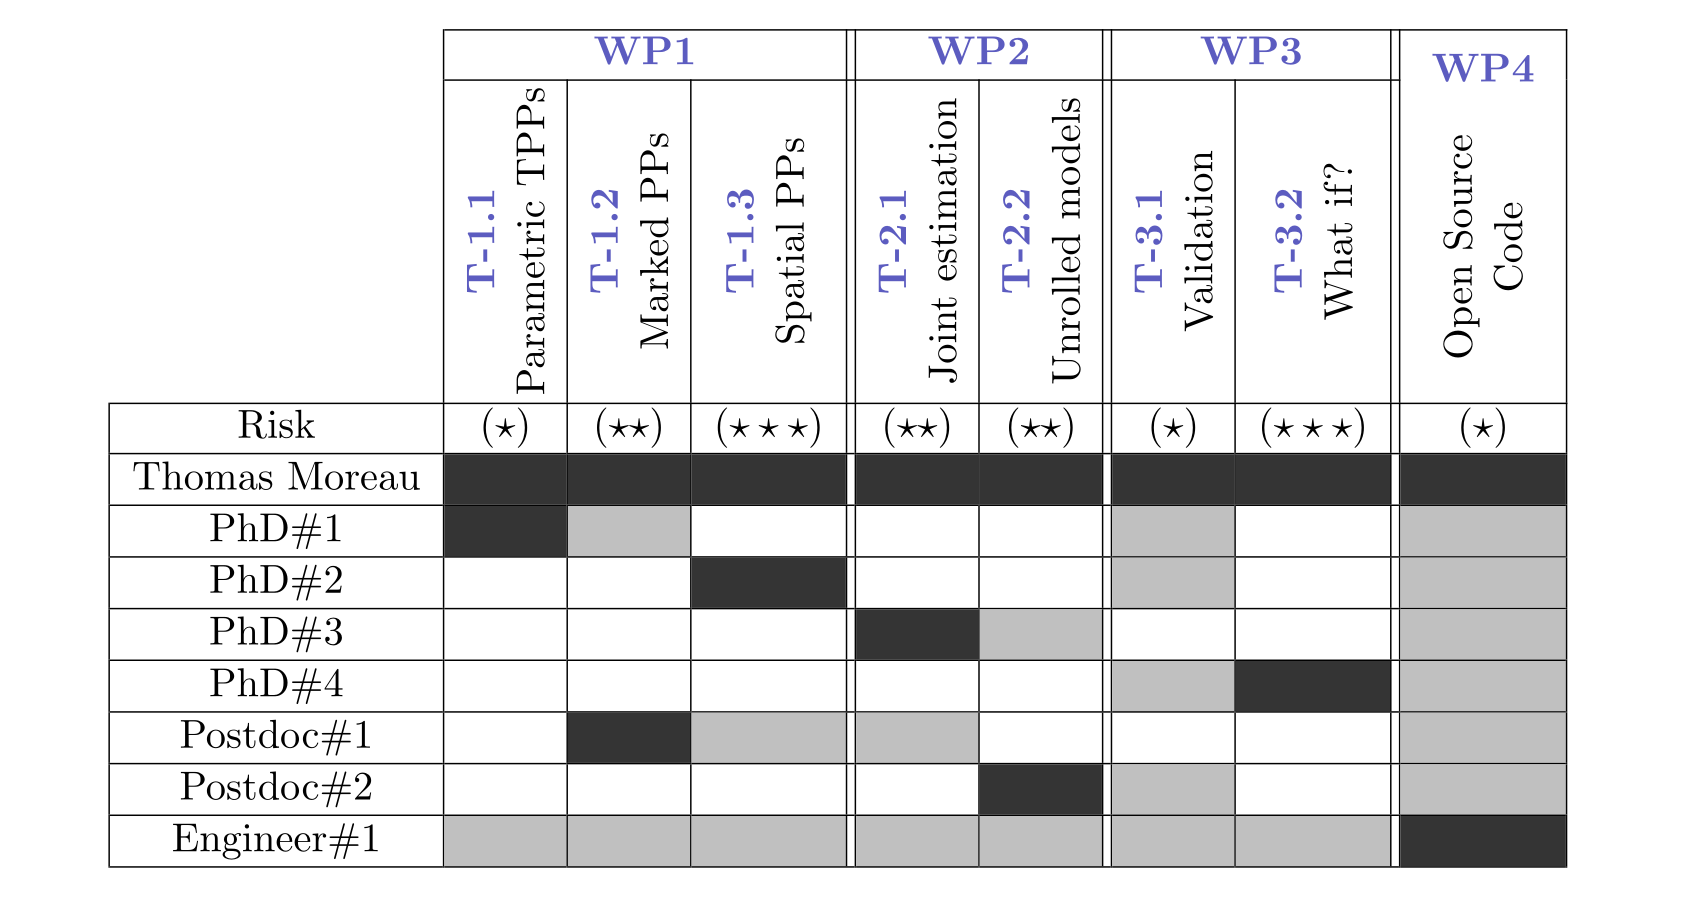
\includegraphics[width=\textwidth]{task_table}\\
}


%------------------------------------------------------------------------------

\begin{frame}[t]{Application domains}

    \vskip-1em
    \begin{columns}[T]
        \column{.5\textwidth}
        \centering
        \begin{tikzpicture}
                \node[inner sep=0em, outer sep=0em] (img) {
                    \includegraphics[width=.8\linewidth]{meg_signal}
                };
                \path let
                  \p1=($(img.north) - (0, 1em)$), \p2=(img.south)
                  in
                  node {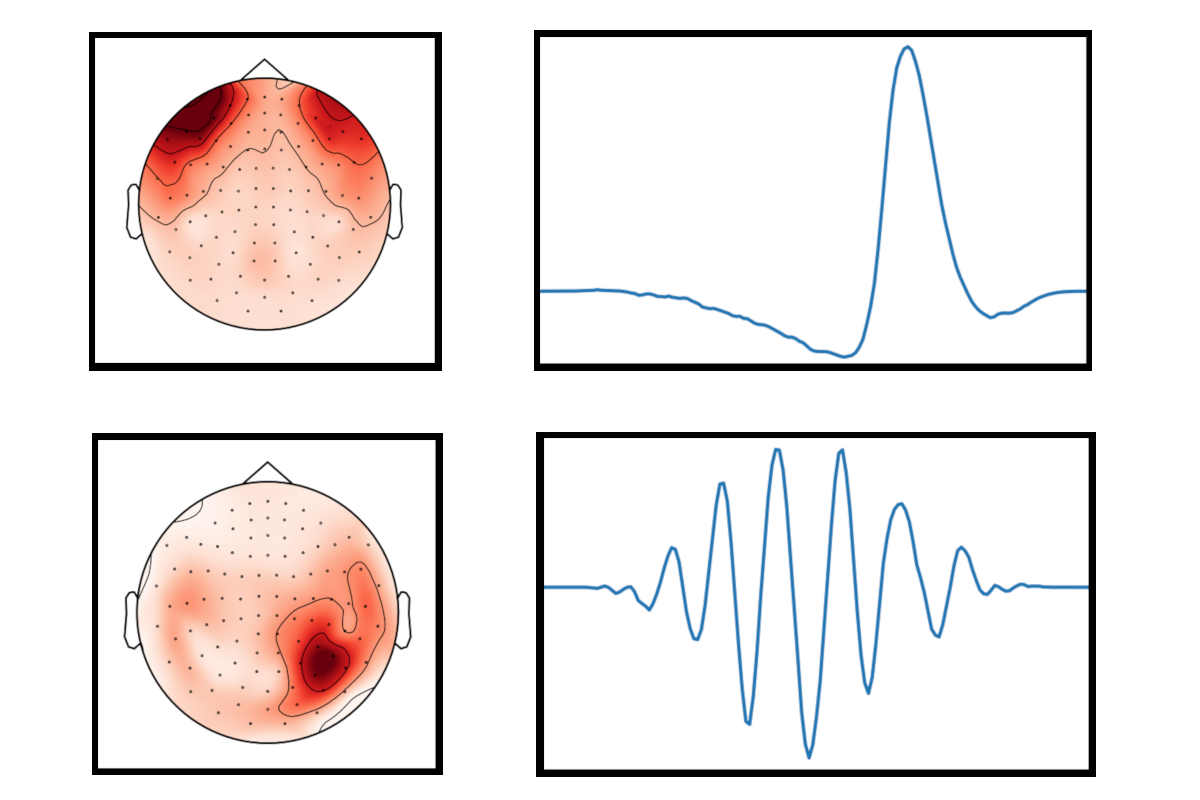
\includegraphics[height=\y1-\y2]{meg_dict}};
            \end{tikzpicture}\\
        {\large Neuroscience (MEG)}\\
        \fakecite{Dupré$^*$, {\bf M.$^*$} et al. NeurIPS 2018}\\[.5em]
        \begin{tikzpicture}
            \node[inner sep=0em, outer sep=0em] (img) {
                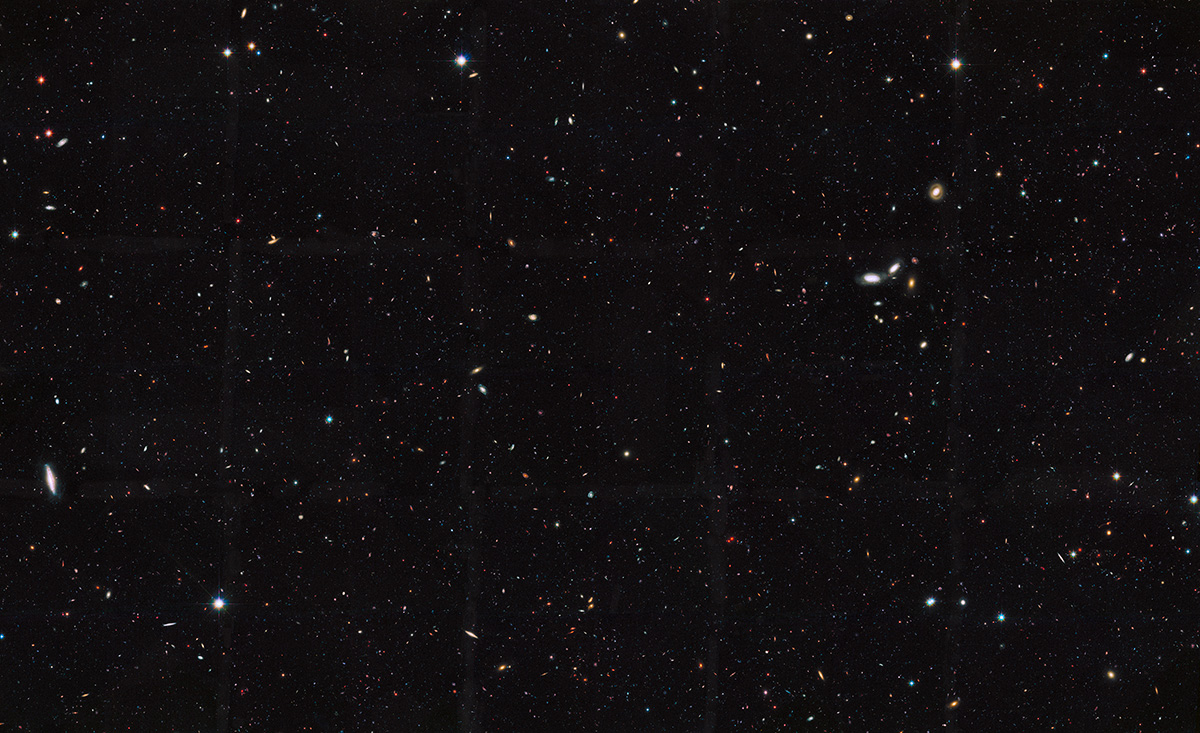
\includegraphics[width=.8\linewidth]{Hubble}
            };
            \path let
                \p1=($(img.north) - (0, 1em)$), \p2=(img.south)
                in
                node {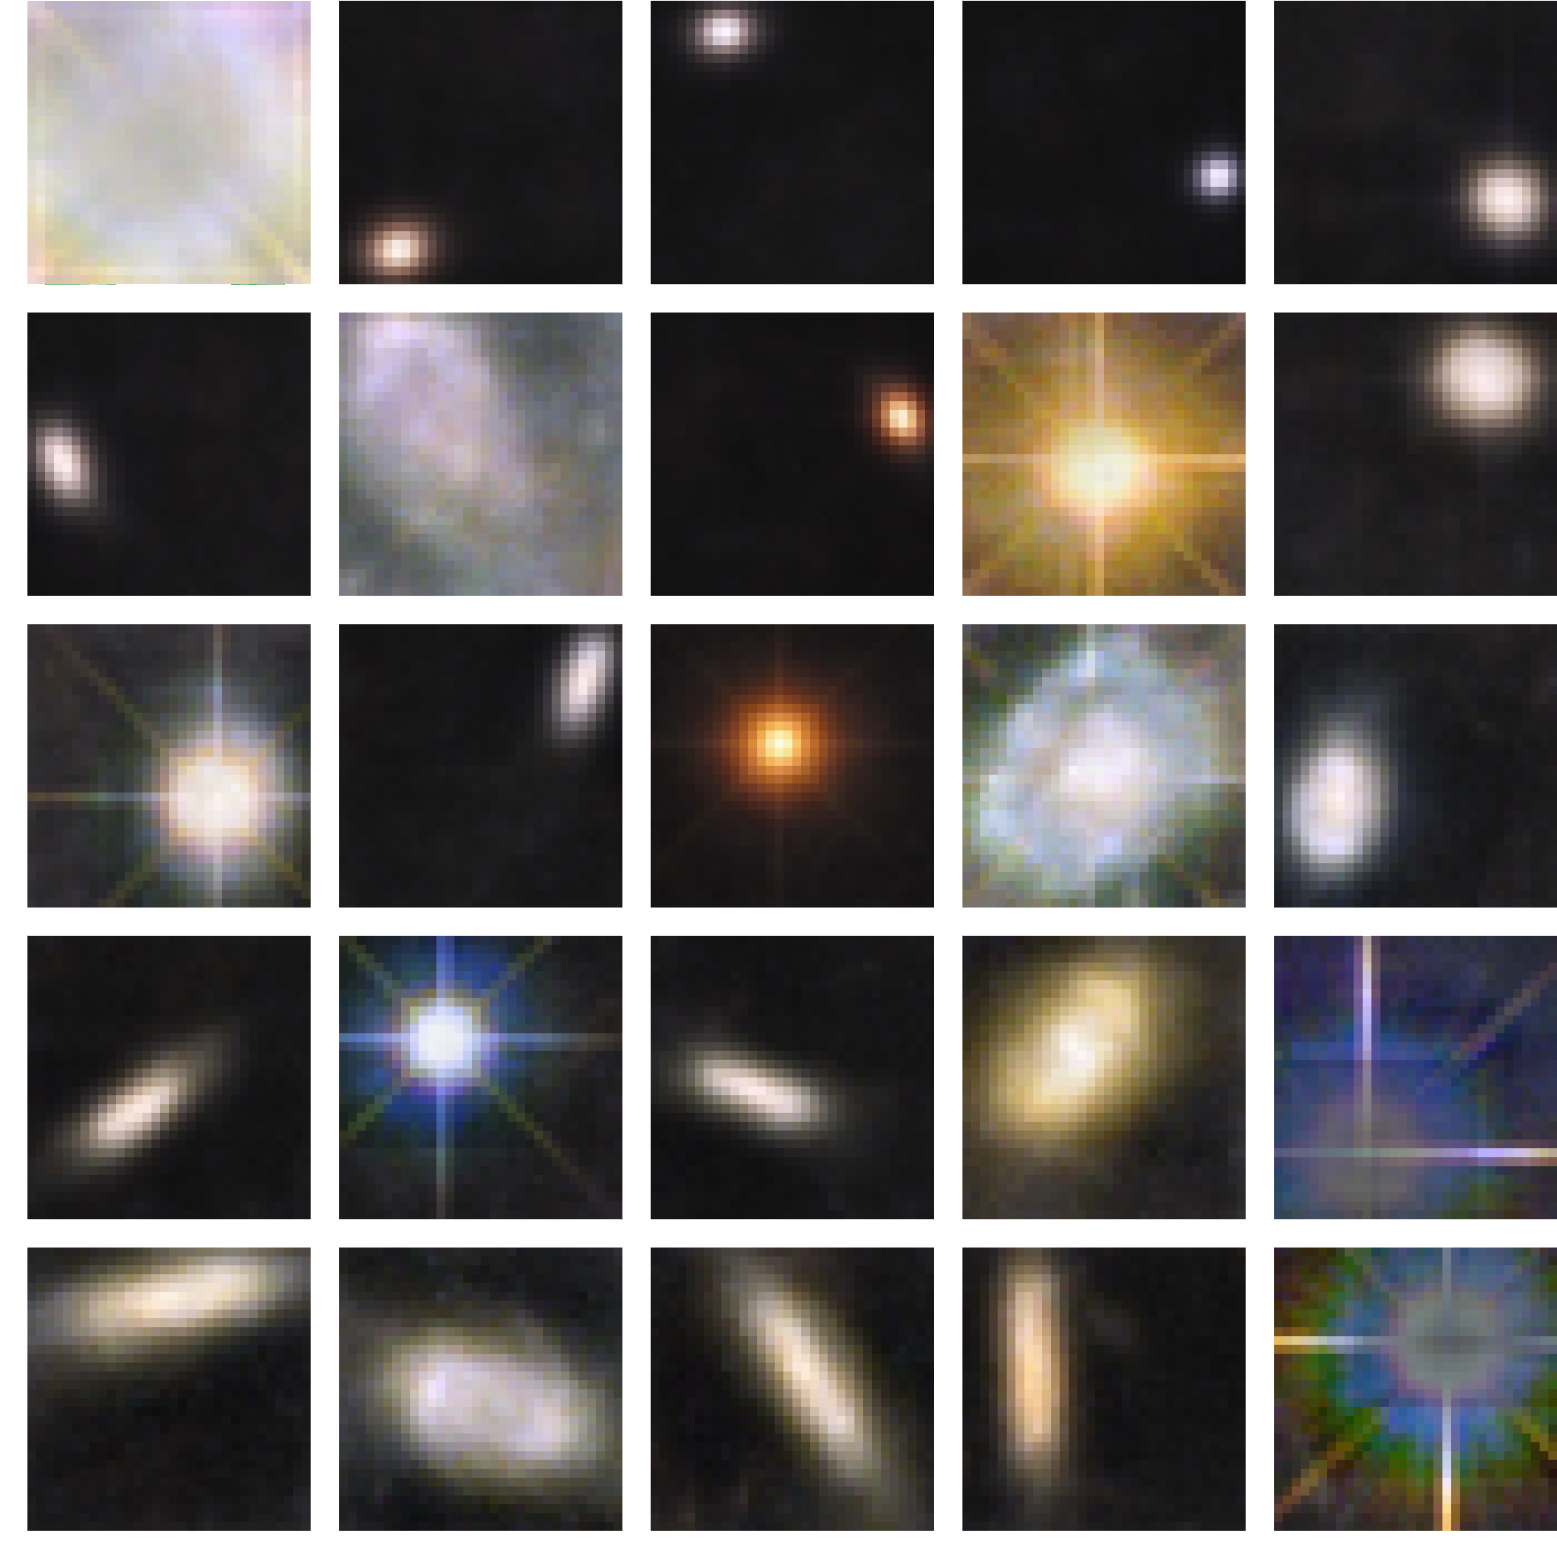
\includegraphics[height=\y1-\y2]{Hubble_dict}};
        \end{tikzpicture}\\
        {\large Astronomy}\\
        \fakecite{{\bf M.} \& Gramfort, PAMI 2020}
    \column{.5\textwidth}
        \centering
        \begin{tikzpicture}
            \node[inner sep=0em, outer sep=0em] (img) {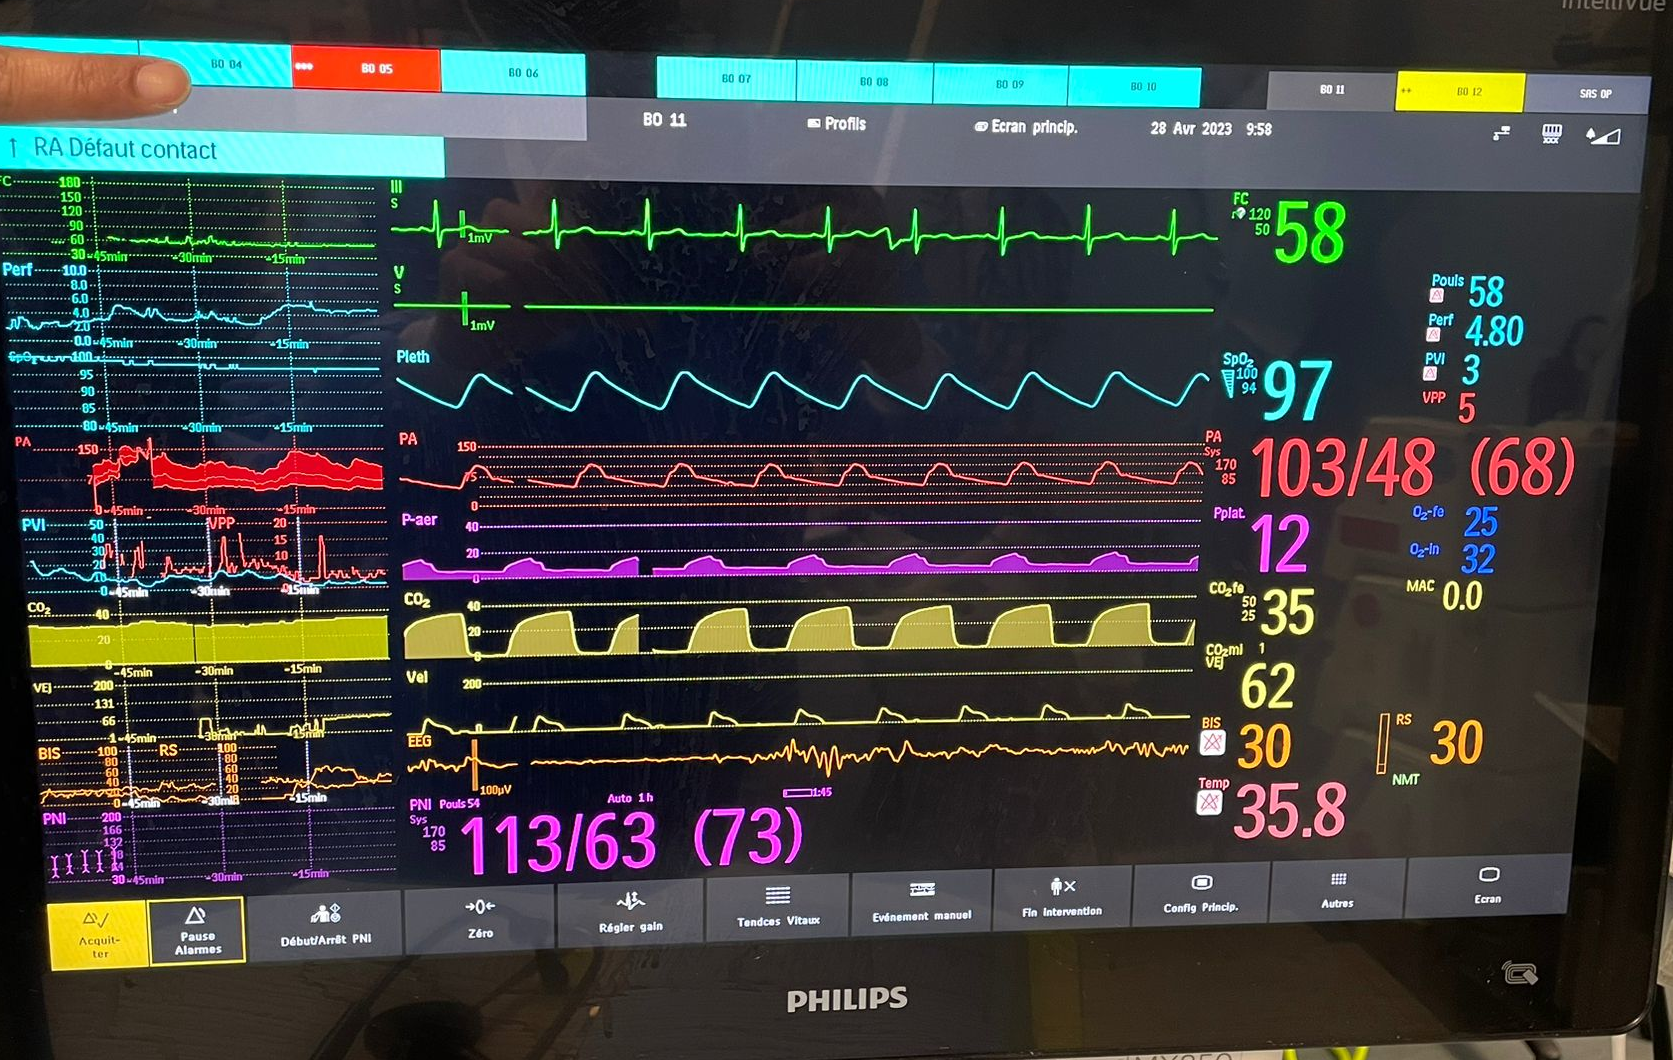
\includegraphics[width=.75\linewidth]{ga_signal}};
            \path let
                \p1=($(img.north) - (0, 1em)$), \p2=(img.south)
                in
                node {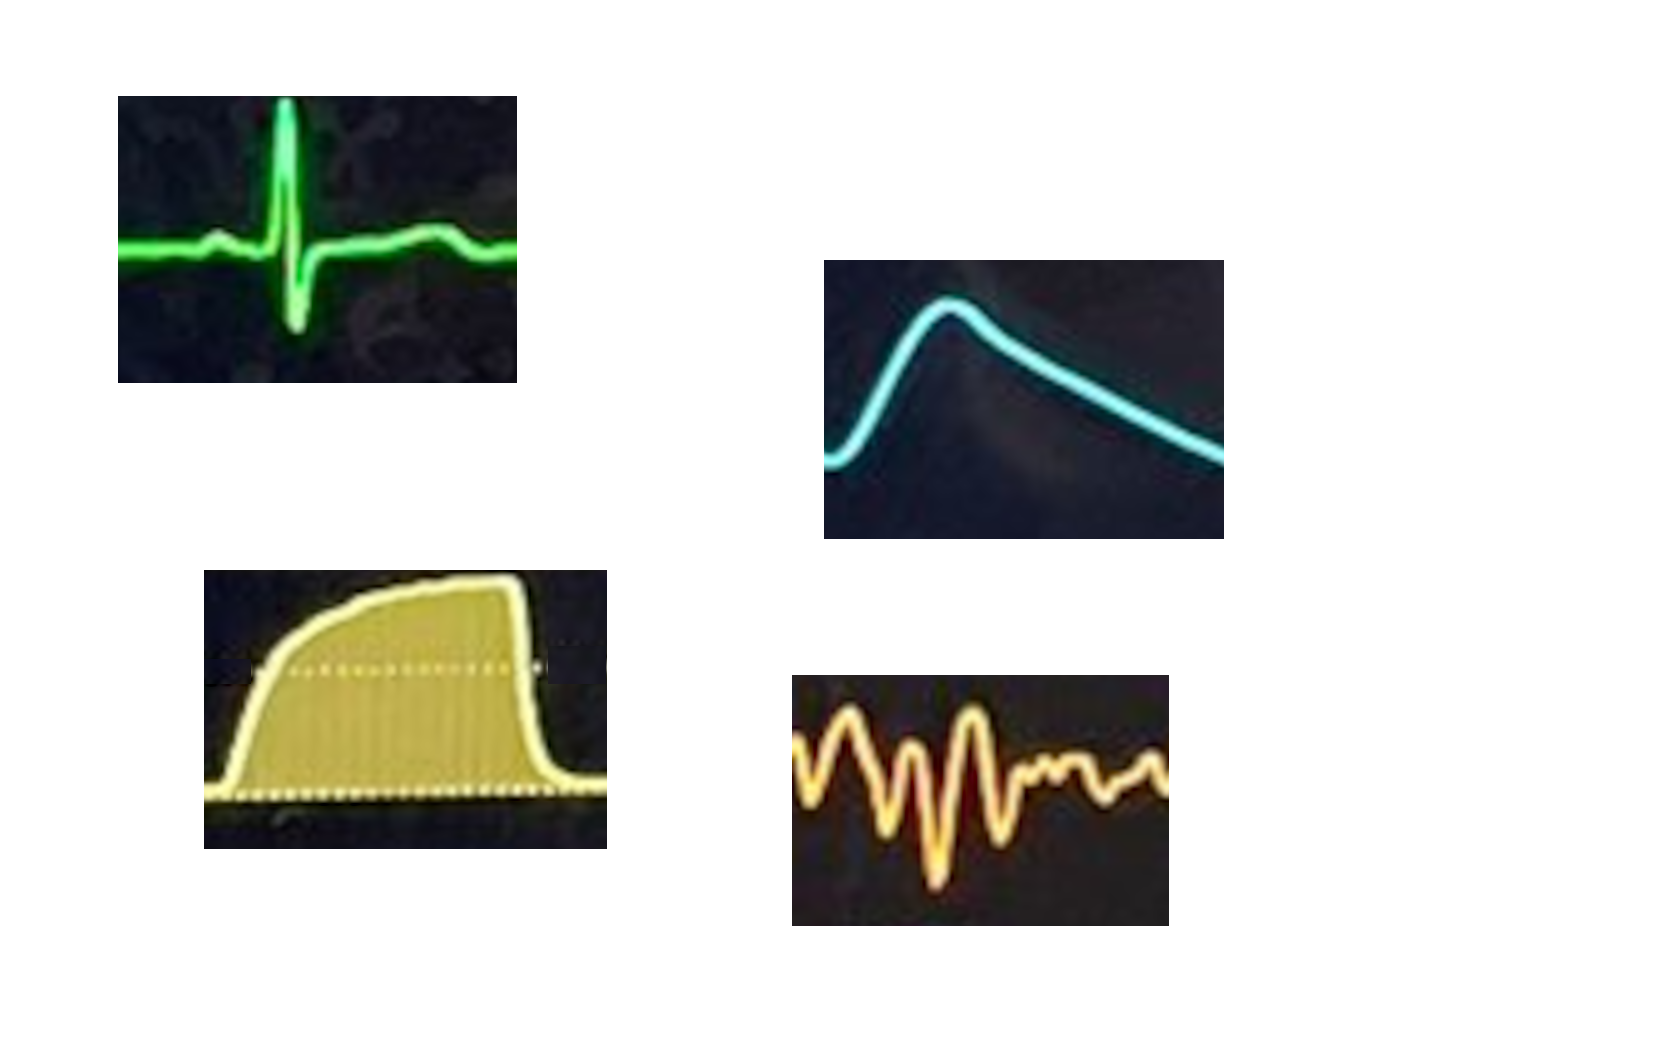
\includegraphics[height=\y1-\y2]{ga_dict}};
        \end{tikzpicture}\\
        {\large General Anesthesia}\\
        \fakecite{Collaboration with Paris Hospitals}\\
        \begin{tikzpicture}
            \node[inner sep=0em, outer sep=0em] (img) {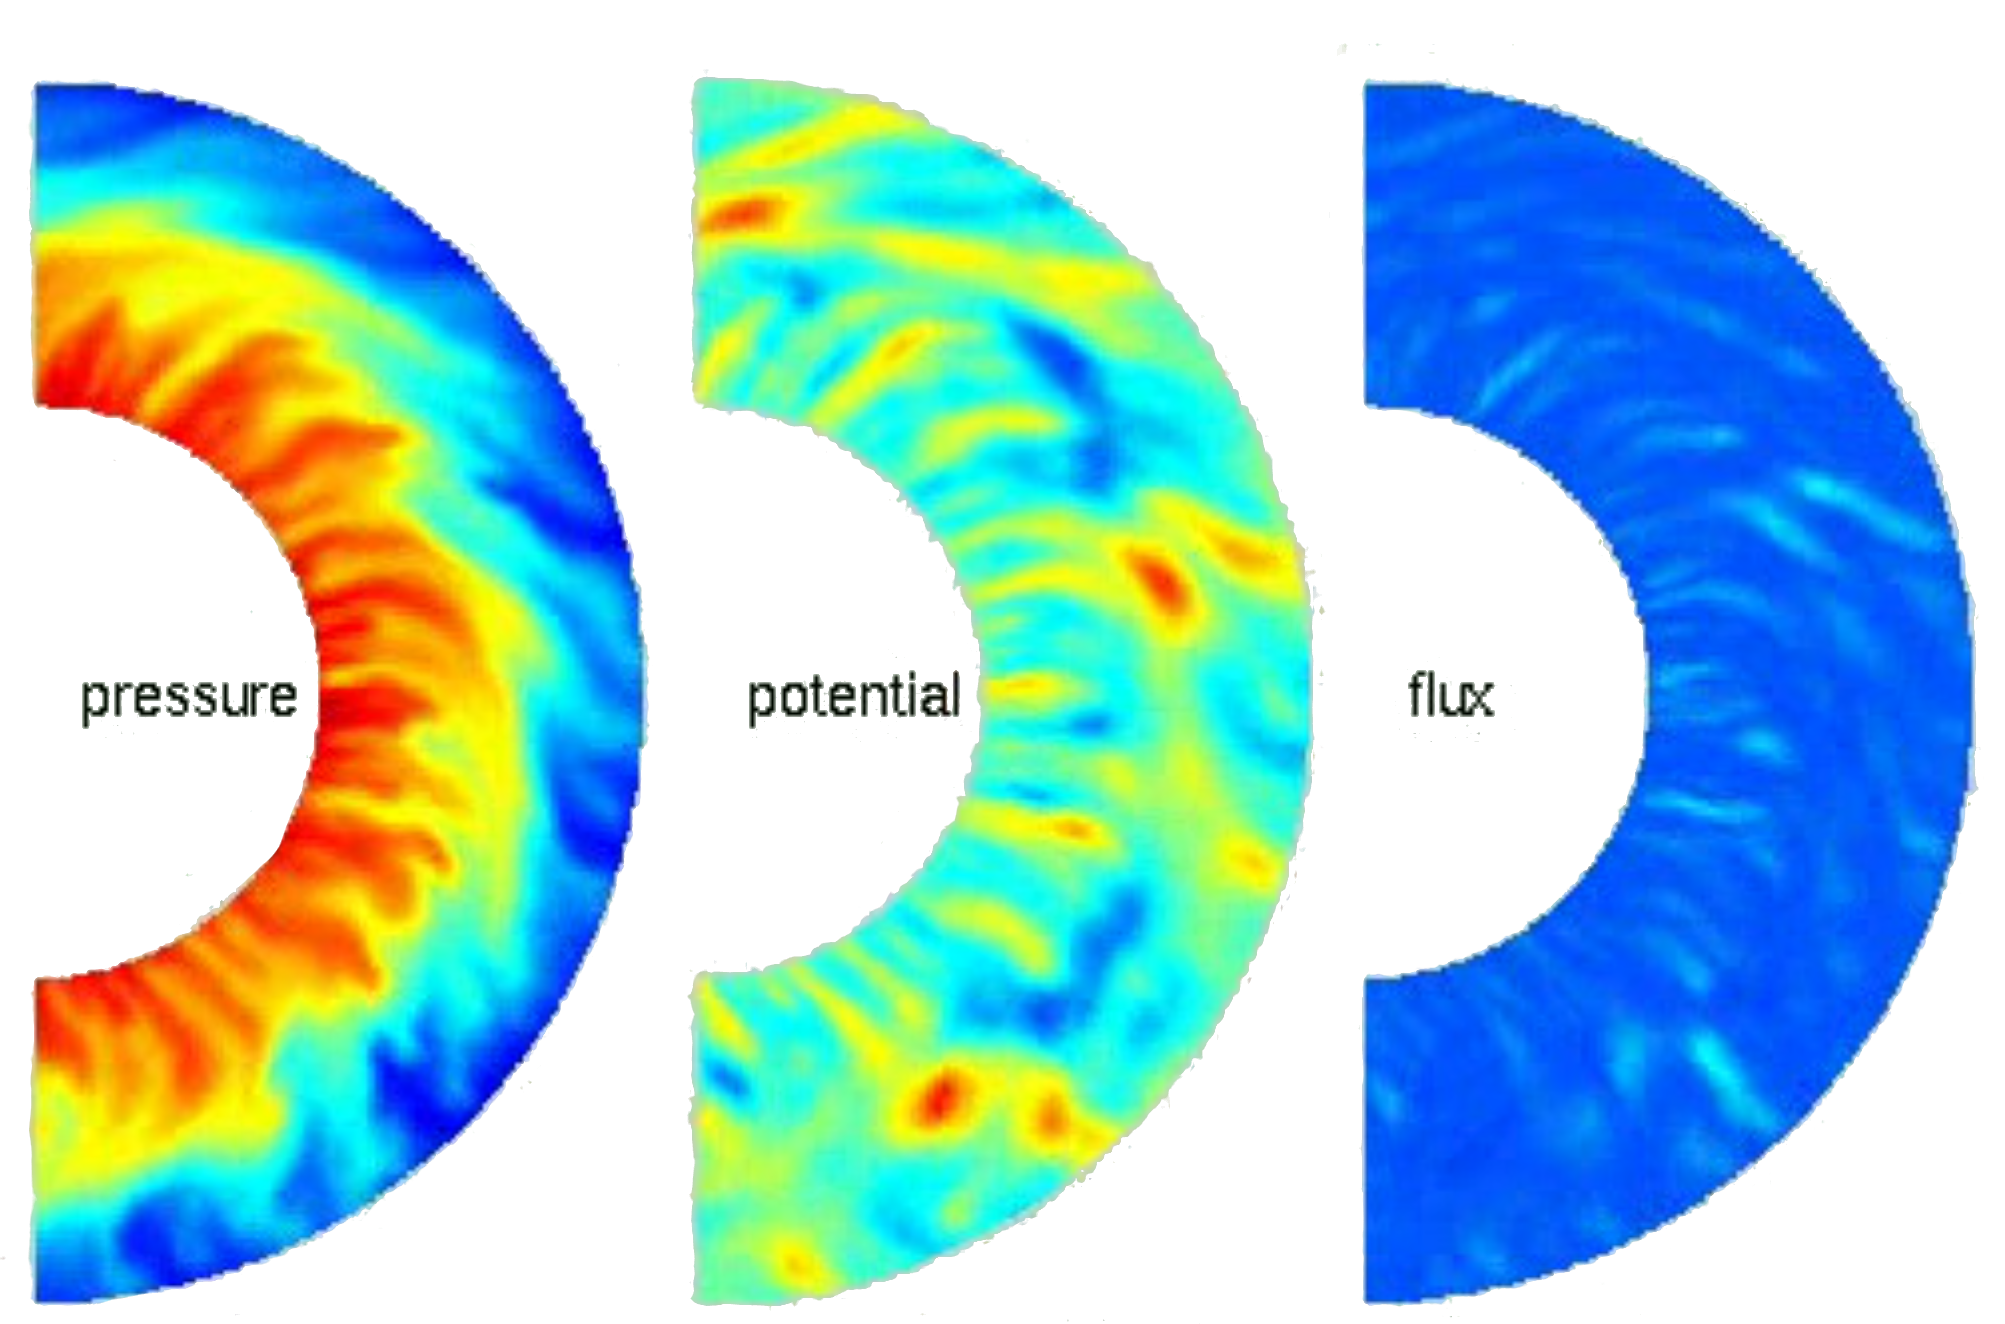
\includegraphics[width=.75\linewidth]{tokamak}};
            \path let
                \p1=($(img.north) - (0, 1em)$), \p2=(img.south)
                in
                node {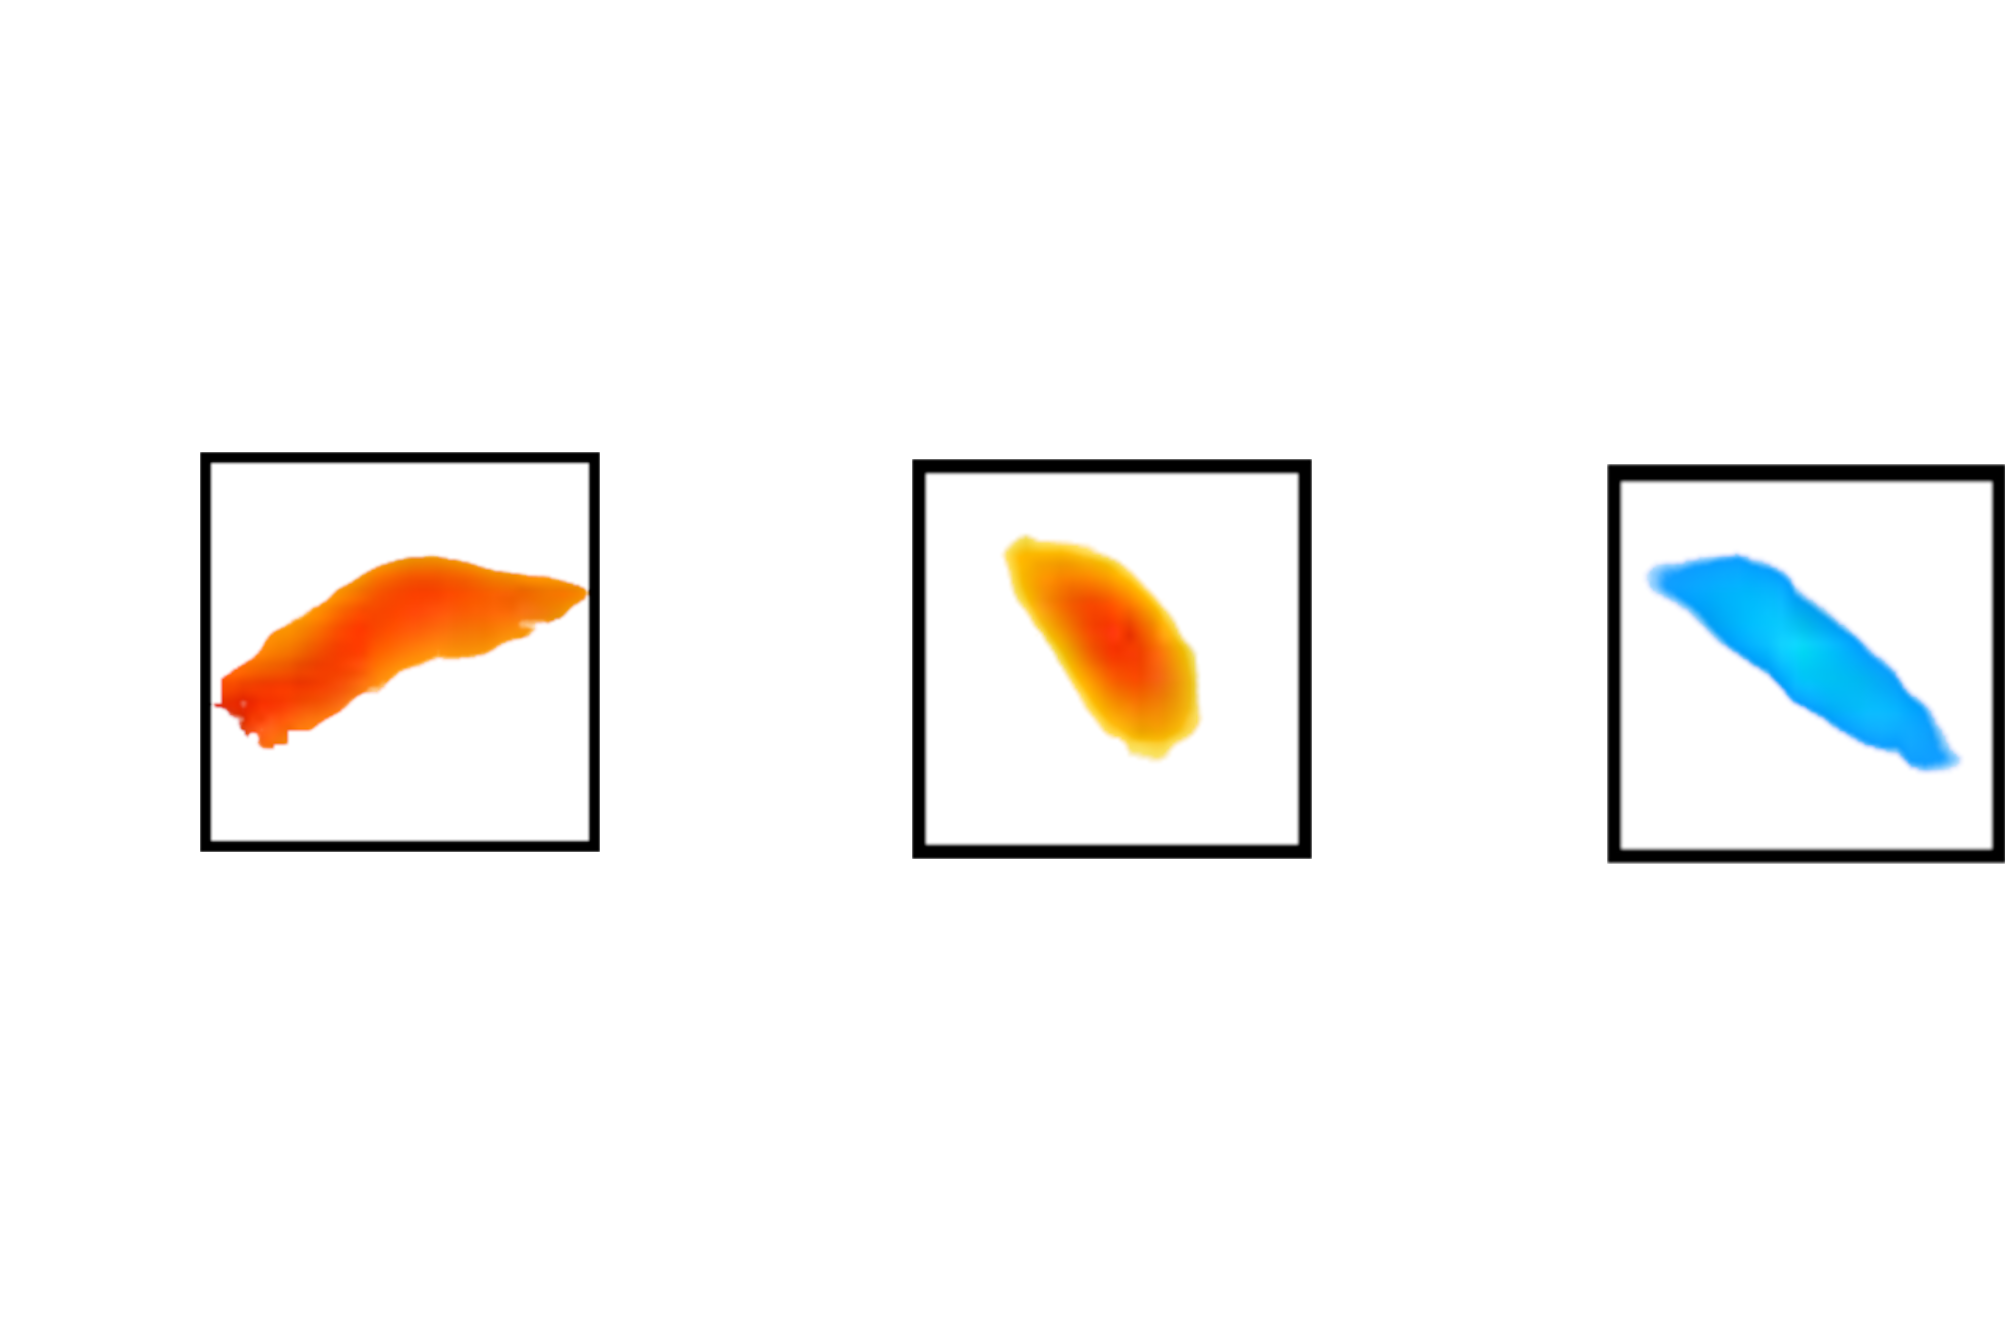
\includegraphics[height=\y1-\y2]{tokamak_dict}};
        \end{tikzpicture}\\
        {\large Physics Simulation}\\
        \fakecite{Collaboration with NumPEx Project}

    \end{columns}
\end{frame}


%------------------------------------------------------------------------------

\frame{
    \frametitle{FaDIn -- PP framework for novel parametric models}

    \myitem{} Opens the way for general parametric PP models\\[.5em]
    \myitem{} Based on discretization and finite support kernel.\\[.5em]
    \myitem{} Efficient inference thanks to pre-computations,\\[.5em]
    \myitem{} Low statistical error,

    \vskip1em

    \centering
    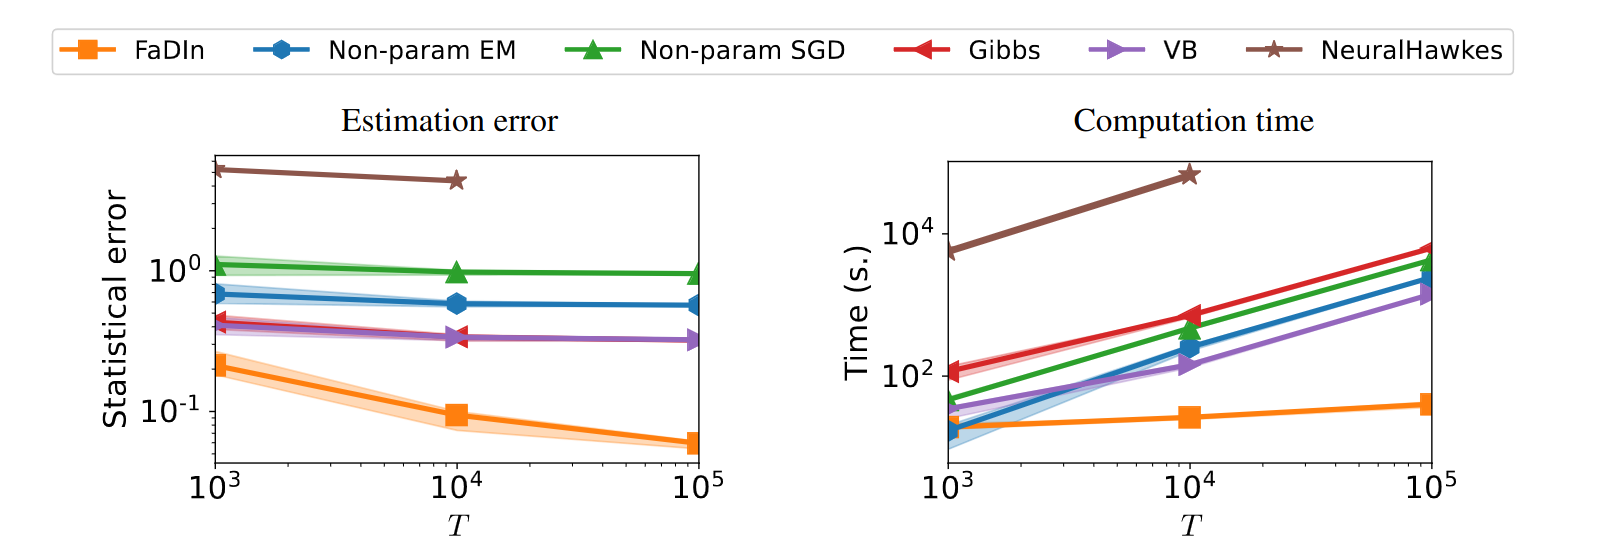
\includegraphics[width=\textwidth]{fadin}\\[.5em]

    \fakecite{Staerman, Allain, Gramfort \& {\bf M.} ICML 2023}

}


\end{document}